\documentclass[12pt]{article}

% =========================
% PAQUETES
% =========================
\usepackage[spanish]{babel}
\usepackage[utf8]{inputenc}
\usepackage[T1]{fontenc}
\usepackage[a4paper, margin=2.5cm]{geometry}
\usepackage{setspace}
\usepackage{graphicx}
\usepackage{longtable}
\usepackage{booktabs}
\usepackage{array}
\usepackage{float}
\usepackage{hyperref}
\usepackage{csquotes}
\usepackage{multirow}

\hypersetup{
	colorlinks=true,
	linkcolor=blue,
	urlcolor=blue
}

\onehalfspacing

% =========================
% BIBLIOGRAFÍA IEEE (DOI CLICKEABLE)
% =========================
\providecommand*{\bibmacro}[2]{}

\usepackage[
style=ieee,
doi=true,
url=false,
backend=biber
]{biblatex}

% DOI limpio y clickeable
\DeclareFieldFormat{doi}{%
	\ifhyperref
	{\href{https://doi.org/#1}{\nolinkurl{#1}}}%
	{#1}%
}


% Mostrar URL solo si no existe DOI
\usepackage{xpatch}
\xpatchbibdriver{article}
{\printfield{url}}
{\iffieldundef{doi}{\printfield{url}}{}}
{}
{}

\addbibresource{referencias_scopus.bib}

% =========================
% TÍTULO
% =========================
\title{
	\begin{flushright}
		\vspace{-2cm}
		
\includegraphics[width=3cm]{Logo/logo.jpg}
	\end{flushright}
	\vspace{-2.8cm}
	
	\textbf{Simulador de Comportamiento Vial con Inteligencia Artificial}\\[6pt]
	{\large Informe Final - Fin de Curso de Ingeniería de Requerimientos}\\[4pt]
}


\author{
	\textbf{Integrantes:}\\
	Panamá Murillo Moisés Antonio\\
	Vera Sánchez Charly Daniel\\
	Zamora Bumbila Diego Alexander\\[6pt]
	\textbf{Carrera:} Ingeniería en Software\\
	\textbf Universidad Técnica Estatal de Quevedo (UTEQ)}

\date{Marzo 2026}

\begin{document}
	\maketitle
	\newpage
	\tableofcontents
	\newpage
	
	% =========================
	\section{Resumen}
	El presente informe corresponde al avance parcial del proyecto fin de curso de la asignatura Ingeniería de Requerimientos.  
	El proyecto plantea el diseño de un \textit{Simulador de Comportamiento Vial con Inteligencia Artificial}, orientado a analizar y mejorar las decisiones de conducción mediante escenarios urbanos simulados y retroalimentación educativa.
	
	Se aplica el enfoque de \textbf{Ingeniería de Requerimientos Orientada a Objetivos (GORE)}, lo que permite identificar metas, subobjetivos y actores del sistema.  
	El documento incluye el árbol jerárquico de objetivos, relaciones de contribución, escenarios de uso, la guía de entrevista estructurada utilizada en la elicitación y el modelado conceptual mediante diagramas UML a nivel de análisis.
	
	% =========================
	\section{Introducción}
	La educación vial tradicional se apoya principalmente en contenidos teóricos, lo que limita la comprensión práctica del comportamiento del conductor frente a situaciones reales de tránsito.  
	Esta limitación se refleja en decisiones incorrectas al conducir y en una mayor probabilidad de incidentes viales, especialmente en conductores en formación.
	
	Ante esta problemática, se plantea el diseño de un simulador inteligente que permita representar escenarios urbanos realistas y analizar el comportamiento vial del usuario.  
	Desde la perspectiva de la Ingeniería de Requerimientos, este informe aborda la fase de análisis, estableciendo las metas del sistema, los actores involucrados y los elementos conceptuales que servirán como base para la especificación de requisitos en etapas posteriores.
    
	\subsection{Descripción del Problema}

El comportamiento de los conductores constituye uno de los factores más determinantes en la ocurrencia de accidentes de tránsito. Diversos estudios han señalado que acciones como el exceso de velocidad, el incumplimiento de señales de tránsito, las maniobras peligrosas y la conducción distraída representan una proporción significativa de los incidentes viales en entornos urbanos.

A pesar de la existencia de normas de tránsito y sistemas de control tradicionales, muchas de estas conductas se producen de manera impredecible y dependen de múltiples variables relacionadas con el contexto, la infraestructura vial y las decisiones individuales de los conductores. Esta complejidad dificulta el análisis sistemático del comportamiento vial y limita la capacidad de evaluar de forma anticipada situaciones de riesgo.

En este contexto, los entornos de simulación constituyen una herramienta útil para estudiar el comportamiento de los conductores bajo diferentes condiciones de tráfico, permitiendo analizar patrones de conducción y evaluar posibles escenarios sin intervenir directamente en sistemas reales.

Sin embargo, muchos simuladores existentes se centran principalmente en la representación visual del entorno o en la dinámica vehicular, dejando en segundo plano el análisis inteligente del comportamiento de los conductores. Esto genera una oportunidad para integrar técnicas de inteligencia artificial que permitan analizar datos de simulación y detectar patrones asociados a conductas de riesgo.

Por esta razón, el presente proyecto plantea el desarrollo conceptual de un sistema de análisis basado en inteligencia artificial aplicado a un simulador de conducción, cuyo propósito es identificar y analizar comportamientos potencialmente peligrosos durante la conducción en escenarios simulados.
	% =========================
	\section{Revisión del Estado del Arte}
	Diversos estudios evidencian el uso de inteligencia artificial y análisis de datos para evaluar el comportamiento del conductor y fortalecer la seguridad vial.  
	Shirole et al.~\cite{Shirole2025} presentan una revisión exhaustiva sobre técnicas de puntuación del comportamiento del conductor basadas en datos, destacando su utilidad para sistemas de evaluación vial.
	
	Investigaciones como las de Harb~\cite{Harb2025} y Almodhwahi y Wang~\cite{Almodhwahi2025} analizan sistemas inteligentes orientados al monitoreo del estado del conductor, mientras que otros trabajos estudian la influencia del entorno vial y patrones de conducción mediante aprendizaje automático y profundo~\cite{Kaselouris202649,Nicolosi2025,Althabhawee2025317}.
	
	Estas investigaciones respaldan la pertinencia del diseño de simuladores inteligentes con fines educativos y preventivos, así como el uso de datos de comportamiento para la evaluación del conductor. En particular, el conjunto de datos multiclase propuesto por Afridi et al.~\cite{Afridi2025} evidencia la relevancia de estructurar sistemas de análisis del comportamiento vial desde una fase de diseño orientada a la clasificación y evaluación de conductas.
	
	% =========================
	\section{Marco de Trabajo de Ingeniería de Requerimientos}
	El proyecto adopta un marco de trabajo de Ingeniería de Requerimientos con un enfoque iterativo inspirado en Scrum, adecuado para el análisis progresivo del dominio del problema.  
	Las principales actividades consideradas son:
	
	\begin{itemize}
		\item Elicitación de requisitos mediante entrevistas estructuradas.
		\item Observación directa del comportamiento de conductores en formación.
		\item Análisis y organización de requisitos funcionales y no funcionales.
		\item Modelado conceptual del sistema.
		\item Validación temprana de metas y requisitos con los actores.
	\end{itemize}
	
	Este marco facilita la trazabilidad entre objetivos, actores y requisitos, sin abordar aún aspectos de implementación.
% =========================
    \section{Metodología de Desarrollo}

El desarrollo del presente proyecto se basa en un enfoque iterativo inspirado en metodologías ágiles y en prácticas de ingeniería de software orientadas a la gestión de requisitos. Este enfoque permite abordar el análisis del sistema de manera progresiva, facilitando la incorporación de nuevos conocimientos sobre el dominio del problema a lo largo del proceso de desarrollo.

Las metodologías ágiles, particularmente Scrum, promueven ciclos de desarrollo cortos y retroalimentación continua entre los participantes del proyecto. No obstante, diversos estudios han señalado que, en la práctica, los equipos de desarrollo suelen complementar Scrum con técnicas formales de ingeniería de software, especialmente en actividades relacionadas con el análisis y la gestión de requisitos \cite{Dada20221429}.

En el contexto de este proyecto, el proceso de desarrollo se apoya en principios de Ingeniería de Requerimientos definidos en estándares y literatura especializada, los cuales enfatizan la importancia de la elicitation, especificación, análisis y validación de requisitos a lo largo del ciclo de vida del sistema \cite{ISO29148,Wiegers2013}.

Bajo esta perspectiva, el proyecto adopta un modelo de desarrollo iterativo en el cual se realizan ciclos sucesivos de análisis y refinamiento de los requisitos del sistema. Este enfoque permite mejorar progresivamente la comprensión del dominio del problema, así como validar los modelos conceptuales del sistema antes de una eventual implementación.

Las principales actividades consideradas dentro de esta metodología incluyen:

\begin{itemize}
\item análisis del dominio del problema y revisión de literatura relacionada;
\item identificación y elicitation de requisitos del sistema;
\item modelado conceptual de los componentes del sistema;
\item definición de escenarios de uso representativos;
\item validación conceptual de los requisitos identificados.
\end{itemize}

Este enfoque metodológico permite estructurar el desarrollo del proyecto manteniendo un equilibrio entre la flexibilidad de los métodos ágiles y la rigurosidad de las prácticas de ingeniería de requisitos.
	% =========================
	\section{Stakeholders}
	
	La identificación de stakeholders permite reconocer a los actores que influyen o se ven
	afectados por el sistema, facilitando la correcta definición de requisitos \cite{Wiegers2013}.
	
	\begin{itemize}
		\item \textbf{Conductor (usuario final):} Interactúa directamente con el simulador y recibe retroalimentación educativa.
		\item \textbf{Instructor de conducción:} Supervisa el desempeño del conductor y valida los resultados obtenidos.
		\item \textbf{Administrador del sistema:} Gestiona usuarios, escenarios y reglas de tránsito.
		\item \textbf{Autoridades de tránsito:} Definen normativas y lineamientos de seguridad vial.
		\item \textbf{Desarrolladores:} Implementan el sistema conforme a los requisitos especificados.
	\end{itemize}
	
	% =========================
	\section{Técnicas de Elicitación de Requisitos}
	
	Para la obtención de requisitos se aplicaron técnicas de elicitación comúnmente utilizadas en Ingeniería de Requerimientos, seleccionadas por su adecuación al dominio del problema \cite{Wiegers2013}.
	
	En este proyecto se emplearon exclusivamente entrevistas estructuradas y observación directa, debido a que permiten obtener información cualitativa profunda y contextualizada sobre el comportamiento vial y las necesidades del sistema.
	
	\subsection{Entrevistas Estructuradas}
	
	Se realizaron entrevistas estructuradas a conductores en formación e instructores de conducción, con el objetivo de identificar necesidades, expectativas y problemáticas frecuentes relacionadas con el aprendizaje vial \cite{Wiegers2013,Levaniuk202549}.
	
	Las entrevistas fueron diseñadas considerando principios de elicitación orientada a metas y seguridad, permitiendo identificar tanto requisitos funcionales como restricciones no funcionales del sistema.
	
	\subsection{Observación Directa}
	
	Se empleó observación directa en sesiones prácticas de conducción, permitiendo identificar patrones de comportamiento, errores recurrentes y situaciones críticas que deben ser modeladas en el simulador \cite{Nicolosi2025}.
	
	Esta técnica facilitó la validación empírica de los escenarios definidos y fortaleció la coherencia entre los objetivos GORE y los requisitos derivados.
	
	% =========================
	\section{Metas y GORE}
	
	\subsection{Meta General}
	\textbf{Evaluar y mejorar el comportamiento vial del conductor mediante la simulación de escenarios urbanos realistas y retroalimentación educativa.}
	
	\subsection{Árbol Jerárquico de Objetivos (GORE)}
	
	\begin{itemize}
		\item \textbf{GOAL:} Mejorar el comportamiento vial del conductor.
		\begin{itemize}
			\item \textbf{SubGoal 1:} Simular escenarios viales realistas.  
			\textbf{Actor:} Desarrolladores
			
			\item \textbf{SubGoal 2:} Evaluar las decisiones del conductor.  
			\textbf{Actor:} Instructor de conducción
			
			\item \textbf{SubGoal 3:} Proporcionar retroalimentación educativa.  
			\textbf{Actor:} Conductor
			
			\item \textbf{SubGoal 4:} Asegurar el rendimiento y fiabilidad del sistema.  
			\textbf{Actor:} Administrador del sistema
			
			\item \textbf{SubGoal 5:} Garantizar la privacidad y seguridad de los datos.  
			\textbf{Actor:} Autoridad de Tránsito
		\end{itemize}
	\end{itemize}
	
	\subsection{Representación Visual del Árbol GORE}
	\begin{figure}[H]
		\centering
		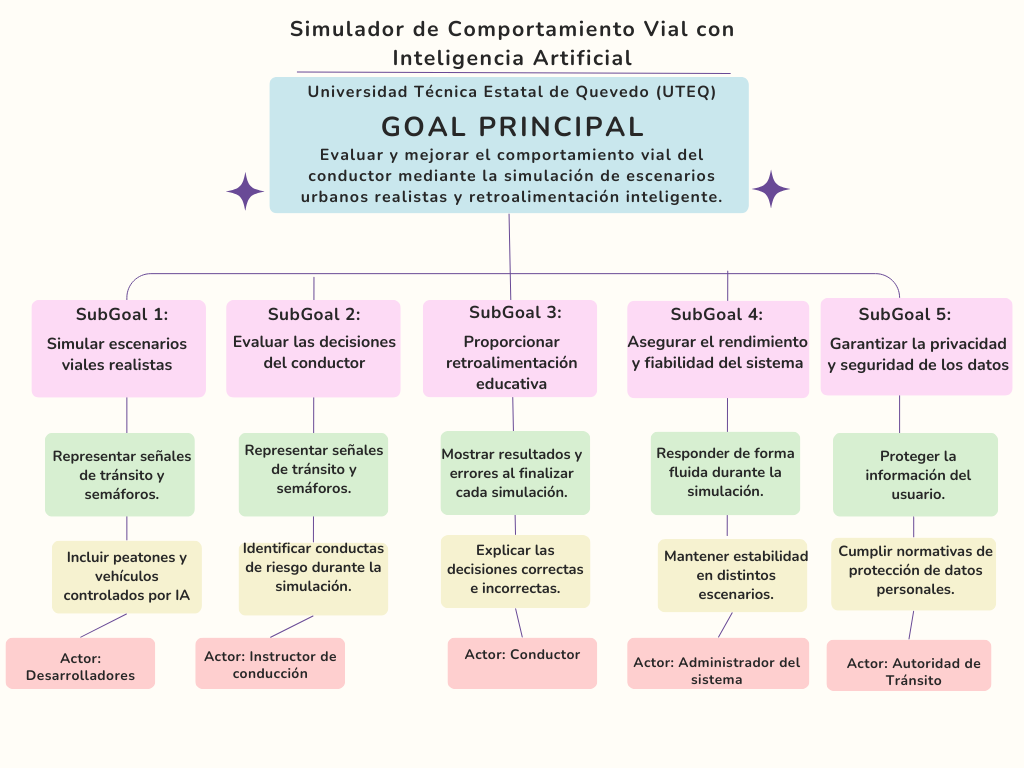
\includegraphics[width=0.9\textwidth]{Arbol gore/arbol.png}
		\caption{Árbol Jerárquico de Objetivos GORE}
	\end{figure}
	
	Los subobjetivos técnicos relacionados con rendimiento, fiabilidad y seguridad se materializan principalmente en requisitos no funcionales definidos posteriormente.
	
	% =========================
	\section{Escenarios}
	
	Los escenarios permiten describir comportamientos esperados del sistema bajo contextos específicos, facilitando la transición hacia casos de uso formales \cite{Holtmann20222171,Koch202215}.
	
	\subsection{Escenario 1: Conducción Normal}
	
	\textbf{Descripción:}  
	El conductor respeta señales de tránsito, mantiene velocidad adecuada y responde correctamente ante peatones.
	
	\textbf{Resultado esperado:}  
	El sistema registra desempeño positivo y genera retroalimentación favorable.
	
	\subsection{Escenario 2: Infracción de Tránsito}
	
	\textbf{Descripción:}  
	El conductor excede el límite de velocidad o ignora una señal de tránsito.
	
	\textbf{Resultado esperado:}  
	El sistema detecta la infracción, actualiza métricas y registra el evento en el historial.
	
	\subsection{Escenario 3: Evaluación Final}
	
	\textbf{Descripción:}  
	Al finalizar la simulación, el sistema procesa las métricas registradas.
	
	\textbf{Resultado esperado:}  
	Se genera un reporte de desempeño y retroalimentación educativa personalizada.
	
	% =========================
	\section{Requisitos Orientados a Soluciones}
	
	De acuerdo con la norma ISO/IEC/IEEE 29148 \cite{ISO29148}, los requisitos deben ser claros, verificables y trazables a los objetivos definidos. En esta fase se establecen requisitos preliminares derivados del análisis GORE y de las técnicas de elicitación aplicadas.
	
	\subsection{Requisitos Funcionales}
	
	\begin{itemize}
		\item RF-01: El sistema deberá permitir la autenticación de usuarios mediante credenciales válidas.
		
		\item RF-02: El sistema deberá permitir seleccionar escenarios de simulación con diferentes niveles de dificultad.
		
		\item RF-03: El sistema deberá simular señales de tránsito, peatones y vehículos en entornos urbanos.
		
		\item RF-04: El sistema deberá registrar en tiempo real las decisiones del conductor.
		
		\item RF-05: El sistema deberá analizar el comportamiento del conductor utilizando un módulo de inteligencia artificial.
		
		\item RF-06: El sistema deberá generar métricas cuantificables de desempeño a partir del análisis realizado por el módulo de inteligencia artificial.
		
		\item RF-07: El sistema deberá proporcionar retroalimentación educativa al finalizar la simulación.
		
		\item RF-08: El sistema deberá almacenar el historial de prácticas del usuario.
		
		\item RF-09: El sistema deberá permitir la generación de reportes de desempeño.
		
		\item RF-10: El sistema deberá permitir al administrador configurar escenarios y reglas de tránsito.
	\end{itemize}
	
	\subsection{Requisitos No Funcionales}
	
	Siguiendo recomendaciones sobre calidad de requisitos no funcionales \cite{Dongmo202523790,Khalid2025}, se identifican los siguientes:
	
	\begin{itemize}
		\item RNF-01: El sistema deberá mantener una latencia inferior a 100 ms durante la simulación.
		
		\item RNF-02: El sistema deberá garantizar disponibilidad mínima del 95\%.
		
		\item RNF-03: El sistema deberá proteger la información del usuario mediante mecanismos de cifrado.
		
		\item RNF-04: El sistema deberá permitir respaldo periódico de datos.
		
		\item RNF-05: La interfaz deberá permitir que un usuario en formación complete una práctica sin asistencia externa tras un máximo de dos sesiones de uso.
		
		\item RNF-06: El sistema deberá soportar al menos 50 usuarios concurrentes.
	\end{itemize}
	% =========================
    \section{Priorización de Requisitos (MoSCoW)}

La técnica MoSCoW se utiliza para priorizar los requisitos del sistema de acuerdo con su nivel de importancia dentro del desarrollo del proyecto. Esta metodología clasifica los requisitos en cuatro categorías: \textit{Must Have} (requisitos indispensables para el funcionamiento del sistema), \textit{Should Have} (requisitos importantes pero no críticos), \textit{Could Have} (requisitos deseables que pueden implementarse si existe disponibilidad de tiempo y recursos) y \textit{Won't Have} (requisitos que no serán implementados en la versión actual del sistema).

La aplicación de esta técnica permite organizar el desarrollo del sistema de simulación de conducción, asegurando que las funcionalidades esenciales sean implementadas en las primeras fases del proyecto.


\begin{table}[H]
\centering
\begin{tabular}{|c|p{8cm}|c|}
\hline
\textbf{ID} & \textbf{Requisito} & \textbf{Prioridad (MoSCoW)} \\
\hline
RF-01 & El sistema deberá permitir la autenticación de usuarios mediante credenciales válidas. & Must \\
\hline
RF-02 & El sistema deberá permitir seleccionar escenarios de simulación con diferentes niveles de dificultad. & Must \\
\hline
RF-03 & El sistema deberá simular señales de tránsito, peatones y vehículos en entornos urbanos. & Must \\
\hline
RF-04 & El sistema deberá registrar en tiempo real las decisiones del conductor durante la simulación. & Must \\
\hline
RF-05 & El sistema deberá analizar el comportamiento del conductor utilizando un módulo de inteligencia artificial. & Should \\
\hline
RF-06 & El sistema deberá generar métricas cuantificables de desempeño a partir del análisis realizado  por el módulo de inteligencia artificial. & Should \\
\hline
RF-07 & El sistema deberá proporcionar retroalimentación educativa al finalizar la simulación. & Should \\
\hline
RF-08 & El sistema deberá almacenar el historial de prácticas del usuario. & Could \\
\hline
RF-09 & El sistema deberá permitir la generación de reportes de desempeño. & Could \\
\hline
RF-10 & El sistema deberá permitir al administrador configurar escenarios y reglas de tránsito. & Should \\
\hline
\end{tabular}
\caption{Priorización de requisitos utilizando el método MoSCoW}
\end{table}
	% =========================
	\section{Modelado Conceptual}
    % =====================================================
\subsection{Diagrama de Secuencia}
% =====================================================

El diagrama de secuencia representa la interacción temporal entre los actores y los componentes principales del sistema durante la ejecución de una sesión de simulación. Este tipo de diagrama permite visualizar el flujo de mensajes intercambiados entre los elementos del sistema, facilitando la comprensión del comportamiento dinámico del simulador.

En el contexto del \textit{Simulador de Comportamiento Vial con Inteligencia Artificial}, el proceso inicia cuando el usuario accede al sistema y selecciona un escenario de conducción. Posteriormente, el simulador carga el entorno virtual correspondiente y habilita la interacción del conductor con el sistema.

Durante la práctica, las decisiones del conductor son registradas por el simulador y enviadas al módulo de Inteligencia Artificial para su análisis. Este módulo procesa la información y evalúa el comportamiento del usuario considerando variables como el respeto a las señales de tránsito, la velocidad de conducción y los tiempos de reacción ante eventos del entorno.

Finalmente, una vez finalizada la sesión, el sistema genera métricas de desempeño y un reporte de retroalimentación educativa que permite al usuario identificar aciertos y posibles mejoras en su comportamiento vial.

\begin{figure}[H]
\centering
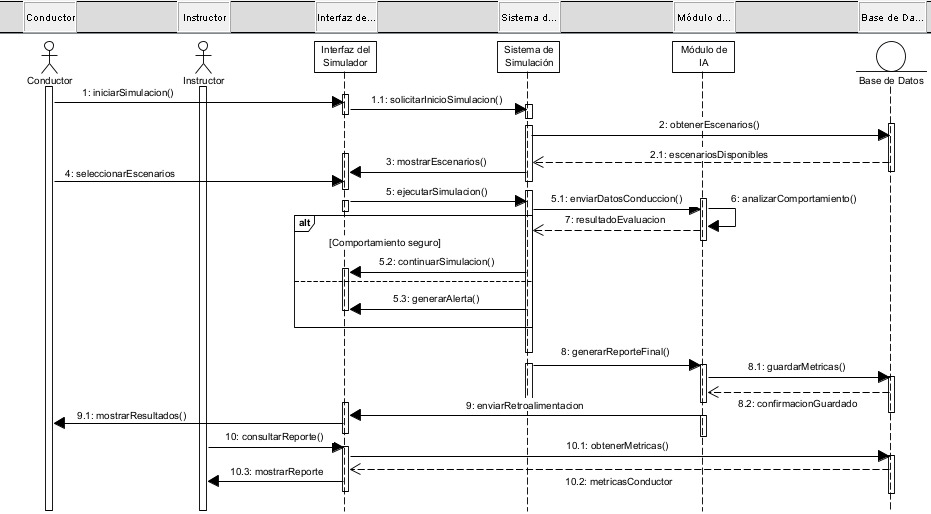
\includegraphics[width=1\textwidth]{Secuencia/secuencia.jpeg}
\caption{Diagrama de Secuencia del simulador vial}
\end{figure}
% =====================================================
\subsection{Diagrama Relacional}
% =====================================================

El diagrama relacional describe la estructura conceptual de los datos utilizados por el sistema y las relaciones existentes entre las principales entidades del simulador. Este modelo permite comprender cómo se organizará la información dentro de la base de datos que soporta el funcionamiento del sistema.

Entre las entidades principales se encuentra el \textit{Usuario}, que representa a los conductores que interactúan con el simulador y realizan las prácticas de conducción. Cada usuario puede ejecutar múltiples sesiones de simulación dentro de diferentes escenarios.

La entidad \textit{Escenario} define las condiciones del entorno vial, incluyendo factores como el tipo de vía, la densidad de tráfico, las condiciones climáticas y el nivel de dificultad. Durante cada sesión de simulación, el sistema registra las acciones realizadas por el conductor y genera métricas de desempeño.

Asimismo, el sistema almacena los \textit{Resultados de Simulación}, los cuales contienen información sobre infracciones detectadas, decisiones tomadas durante la conducción y evaluaciones generadas por el módulo de Inteligencia Artificial.

Este modelo relacional constituye una base conceptual para el posterior diseño de la base de datos del sistema, permitiendo garantizar la correcta organización y trazabilidad de la información generada durante las simulaciones.

\begin{figure}[H]
\centering
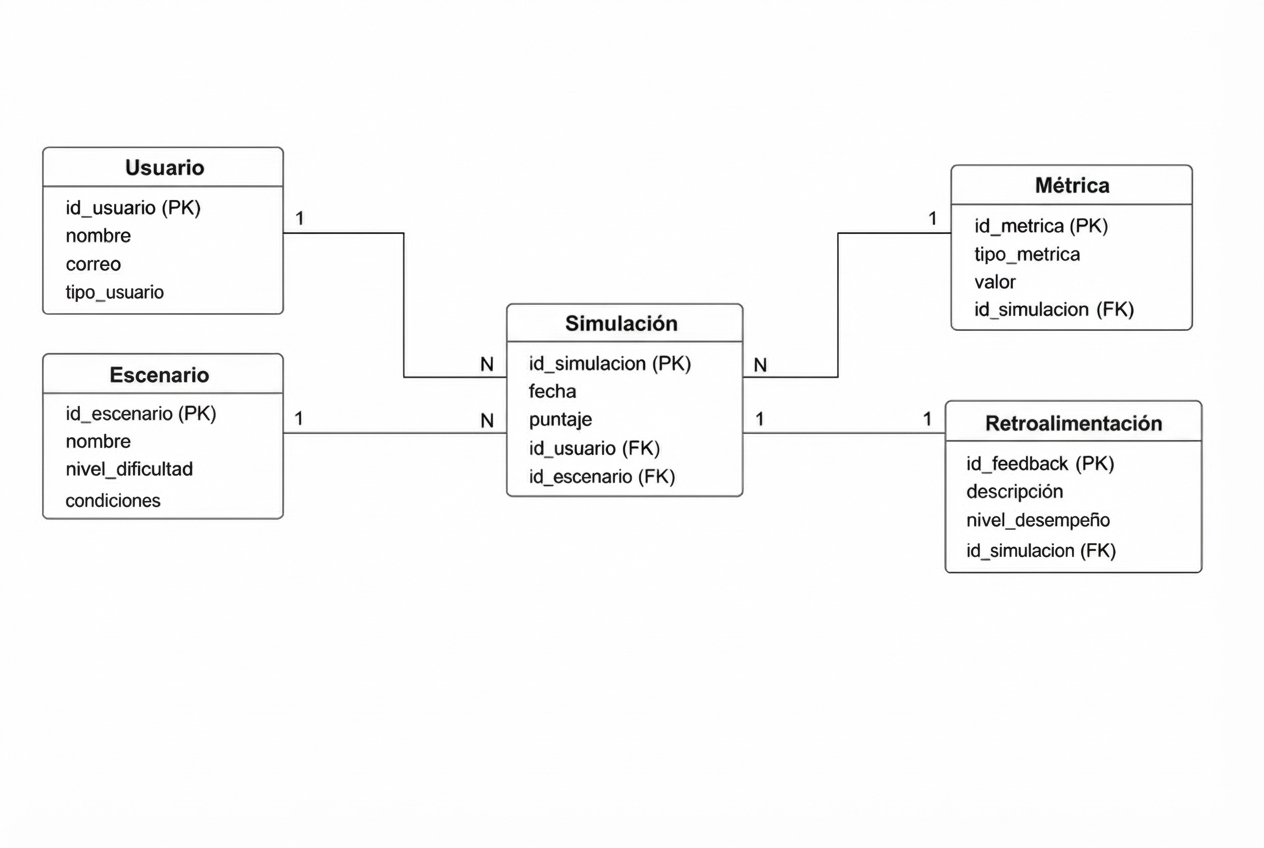
\includegraphics[width=0.9\textwidth]{Relacional/relacional.png}
\caption{Diagrama Relacional del simulador vial}
\end{figure}
	% =========================
	\subsection{Diagrama de Casos de Uso}
	
	\noindent
	\textbf{Actores del Sistema}
	\begin{itemize}
		\item \textbf{Usuarios} – Interactúa con el simulador, realiza prácticas y recibe retroalimentación.
		\item \textbf{Administrador} – Configura escenarios, gestiona usuarios y actualiza reglas de tránsito.
		\item \textbf{IA (Agente externo)} – Analiza decisiones y genera retroalimentación automática.
		\item \textbf{Base de Datos (Agente externo)} – Almacena usuarios, escenarios, métricas y recompensas.
	\end{itemize}

	\begin{figure}[H]
		\centering
		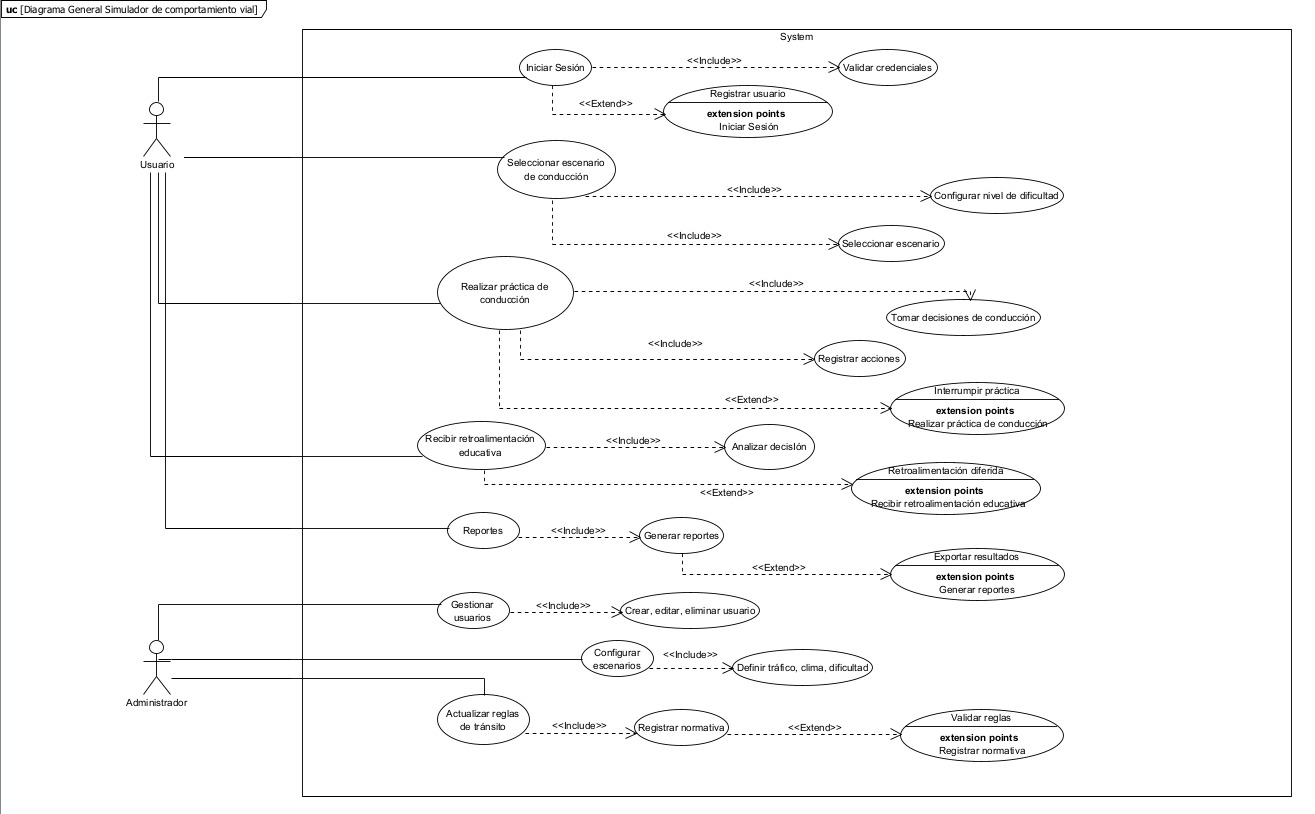
\includegraphics[width=0.9\textwidth]{Casos de uso/general.jpeg}
		\caption{Diagrama de Casos de Uso (nivel análisis)}
	\end{figure}
	
	% =====================================================
	\subsection{Diagramas Individuales de Casos de Uso}
	% =====================================================
	
	Con el propósito de detallar gráficamente la interacción específica de los actores con el sistema, se presentan los diagramas individuales correspondientes a los cinco primeros casos de uso principales del simulador.
	
	Estos diagramas permiten visualizar de forma aislada las relaciones <<include>> y <<extend>>, así como la participación de agentes externos como la IA y la Base de Datos.
	
	% =====================================================
\subsubsection*{CU-01: Iniciar Sesión}
% =====================================================

\begin{figure}[H]
	\centering
	
\includegraphics[width=\textwidth,height=0.85\textheight,keepaspectratio]{Casos de uso/caso1.jpeg}
	\caption{Diagrama de Caso de Uso – Iniciar Sesión. Este diagrama representa el proceso de autenticación del usuario, incluyendo la validación de credenciales con la Base de Datos y la posible extensión hacia el registro de un nuevo usuario en caso de error.}
\end{figure}

% =====================================================
\subsubsection*{CU-02: Seleccionar Escenario de Conducción}
% =====================================================

\begin{figure}[H]
	\centering
	
\includegraphics[width=\textwidth,height=0.85\textheight,keepaspectratio]{Casos de uso/caso2.jpeg}
	\caption{Diagrama de Caso de Uso – Seleccionar Escenario. El diagrama muestra la interacción del usuario con el sistema para elegir un entorno de práctica, incluyendo la consulta obligatoria a la Base de Datos para recuperar los escenarios disponibles.}
\end{figure}

% =====================================================
\subsubsection*{CU-03: Realizar Práctica de Conducción}
% =====================================================

\begin{figure}[H]
	\centering
	
\includegraphics[width=\textwidth,height=0.85\textheight,keepaspectratio]{Casos de uso/caso3.jpeg}
	\caption{Diagrama de Caso de Uso – Realizar Práctica. Este caso de uso representa la ejecución central del simulador, donde el usuario interactúa con el entorno y el sistema registra las decisiones tomadas durante la práctica.}
\end{figure}

% =====================================================
\subsubsection*{CU-04: Recibir Retroalimentación Automática}
% =====================================================

\begin{figure}[H]
	\centering
	
\includegraphics[width=\textwidth,height=0.85\textheight,keepaspectratio]{Casos de uso/caso4.jpeg}
	\caption{Diagrama de Caso de Uso – Recibir Retroalimentación. En este diagrama se observa la participación del módulo de Inteligencia Artificial, encargado de analizar el desempeño y generar el informe pedagógico correspondiente.}
\end{figure}

% =====================================================
\subsubsection*{CU-05: Consultar Puntuación y Métricas}
% =====================================================

\begin{figure}[H]
	\centering
	
\includegraphics[width=\textwidth,height=0.85\textheight,keepaspectratio]{Casos de uso/caso5.jpeg}
	\caption{Diagrama de Caso de Uso – Consultar Métricas. Este caso de uso permite al usuario revisar su historial de desempeño, generando reportes estadísticos almacenados en la Base de Datos.}
\end{figure}

% =====================================================
\subsubsection*{CU-06: Asignación de Recompensas}
% =====================================================

\begin{figure}[H]
	\centering
	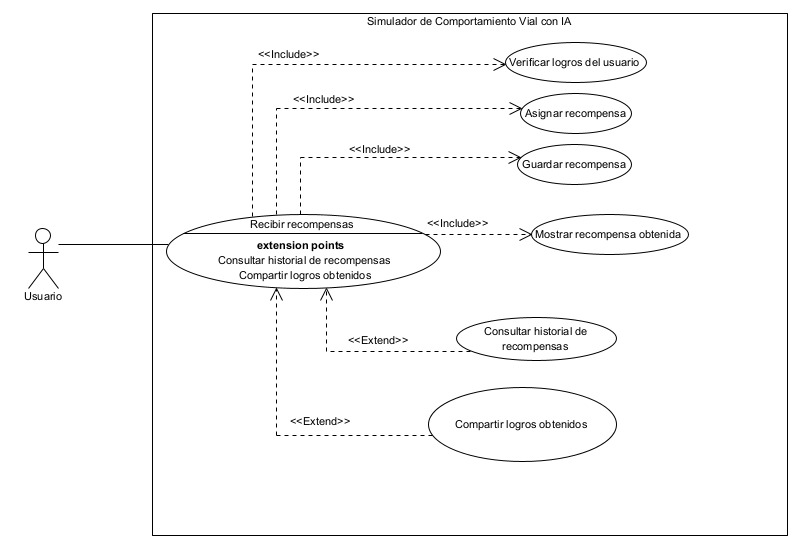
\includegraphics[width=\textwidth,height=0.85\textheight,keepaspectratio]{Casos de uso/caso6.jpeg}
	\caption{Diagrama de Caso de Uso – Asignación de Recompensas. Este caso de uso representa el proceso mediante el cual el sistema evalúa el desempeño del usuario y otorga recompensas o logros según los resultados obtenidos durante las prácticas.}
\end{figure}

% =====================================================
\subsubsection*{CU-07: Configurar Escenarios de Simulación}
% =====================================================

\begin{figure}[H]
	\centering
	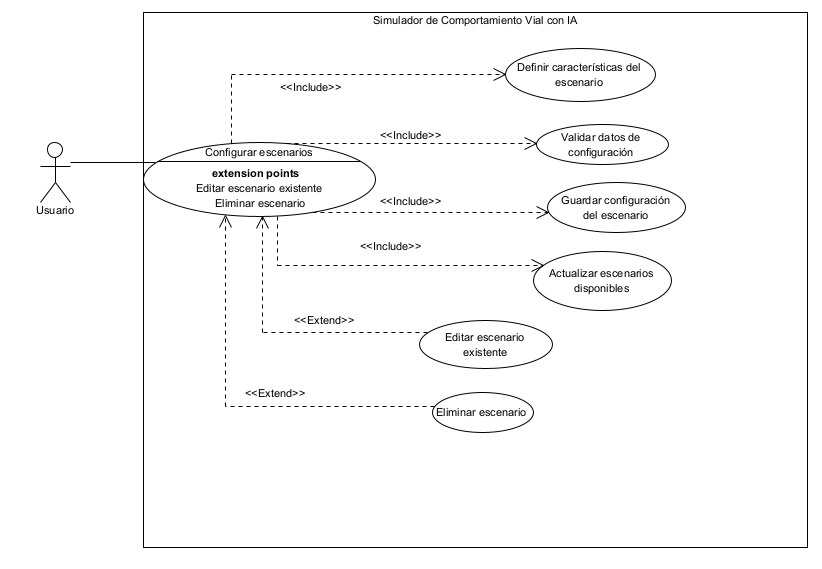
\includegraphics[width=\textwidth,height=0.85\textheight,keepaspectratio]{Casos de uso/caso7.jpeg}
	\caption{Diagrama de Caso de Uso – Configurar Escenarios. En este diagrama se muestra la interacción del administrador con el sistema para crear, modificar o eliminar escenarios de simulación que serán utilizados por los usuarios durante las prácticas.}
\end{figure}

% =====================================================
\subsubsection*{CU-08: Gestionar Normativas de Tránsito}
% =====================================================

\begin{figure}[H]
	\centering
	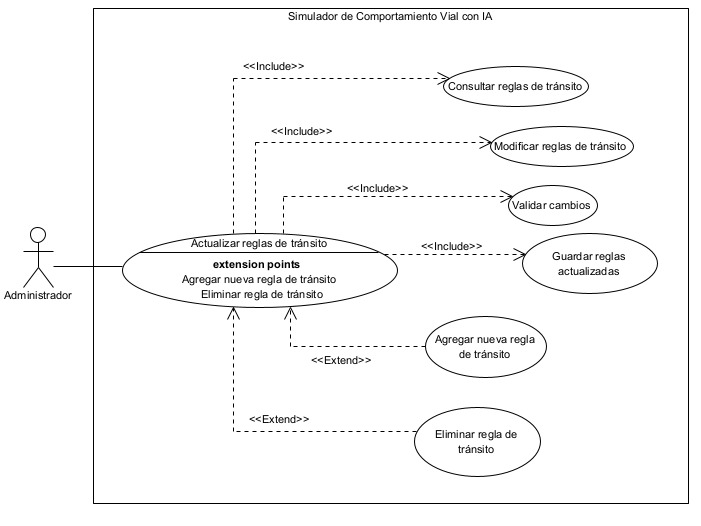
\includegraphics[width=\textwidth,height=0.85\textheight,keepaspectratio]{Casos de uso/caso8.jpeg}
	\caption{Diagrama de Caso de Uso – Gestionar Normativas. Este caso de uso describe el proceso mediante el cual el administrador actualiza y gestiona las reglas de tránsito almacenadas en la Base de Datos, utilizadas por el sistema para evaluar el comportamiento del usuario.}
\end{figure}
% =====================================================
\subsection{Diagramas Individuales de Actividad}
	% =====================================================
% =====================================================
\subsubsection*{DA-01: Inicio de Sesión}
% =====================================================

\begin{figure}[H]
	\centering
	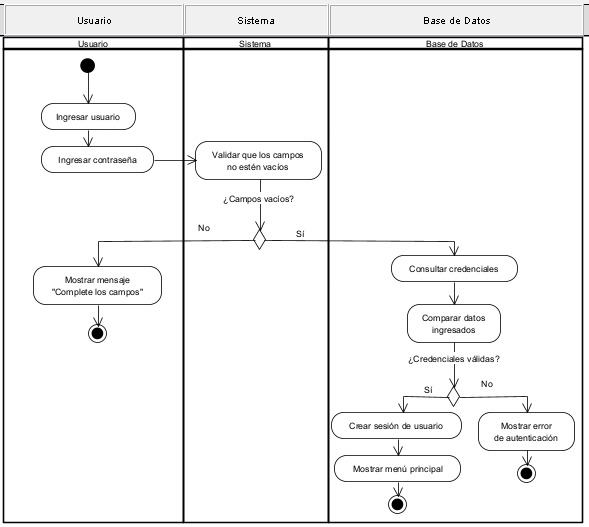
\includegraphics[width=\textwidth,height=0.85\textheight,keepaspectratio]{Actividad/actividad1.jpeg}
	\caption{Diagrama de Actividad – Inicio de Sesión. Este diagrama describe el flujo del proceso de autenticación del usuario dentro del sistema.}
\end{figure}

% =====================================================
\subsubsection*{DA-02: Selección de Escenario}
% =====================================================

\begin{figure}[H]
	\centering
	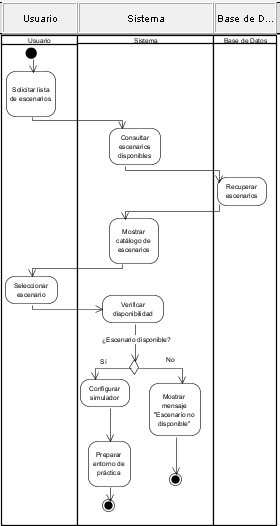
\includegraphics[width=\textwidth,height=0.85\textheight,keepaspectratio]{Actividad/actividad2.jpeg}
	\caption{Diagrama de Actividad – Selección de Escenario. Este diagrama muestra el proceso mediante el cual el usuario selecciona un escenario disponible para la simulación.}
\end{figure}

% =====================================================
\subsubsection*{DA-03: Ejecución de Simulación}
% =====================================================

\begin{figure}[H]
	\centering
	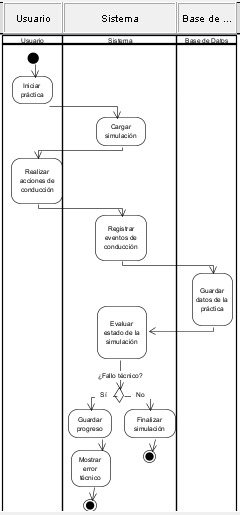
\includegraphics[width=\textwidth,height=0.85\textheight,keepaspectratio]{Actividad/actividad3.jpeg}
	\caption{Diagrama de Actividad – Ejecución de Simulación. Este diagrama representa el flujo de acciones realizadas durante la práctica dentro del simulador.}
\end{figure}

% =====================================================
\subsubsection*{DA-04: Generación de Retroalimentación}
% =====================================================

\begin{figure}[H]
	\centering
	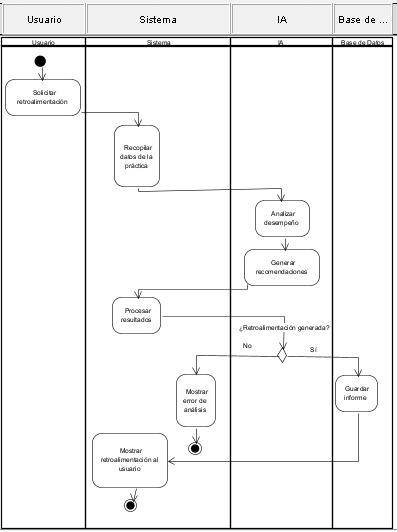
\includegraphics[width=\textwidth,height=0.85\textheight,keepaspectratio]{Actividad/actividad4.jpeg}
	\caption{Diagrama de Actividad – Generación de Retroalimentación. Este diagrama muestra cómo el sistema analiza los resultados de la simulación y genera recomendaciones.}
\end{figure}

% =====================================================
\subsubsection*{DA-05: Consulta de Puntuación y Métricas}
% =====================================================

\begin{figure}[H]
	\centering
	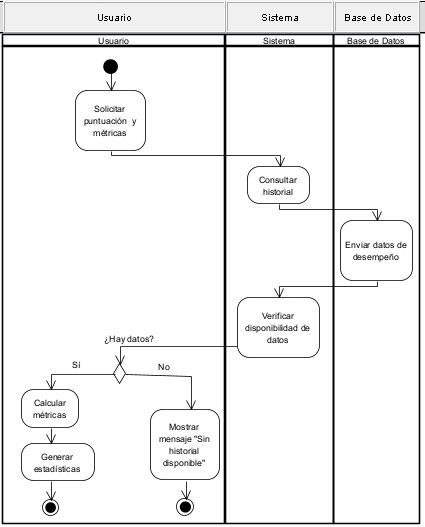
\includegraphics[width=\textwidth,height=0.85\textheight,keepaspectratio]{Actividad/actividad5.jpeg}
	\caption{Diagrama de Actividad – Consulta de Puntuación y Métricas. Este diagrama describe el proceso mediante el cual el usuario consulta sus resultados y estadísticas de desempeño.}
\end{figure}

% =====================================================
\subsubsection*{DA-06: Asignación de Recompensas}
% =====================================================

\begin{figure}[H]
	\centering
	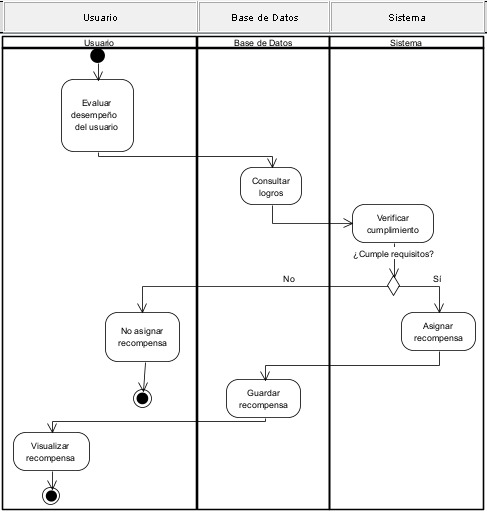
\includegraphics[width=\textwidth,height=0.85\textheight,keepaspectratio]{Actividad/actividad6.jpeg}
	\caption{Diagrama de Actividad – Asignación de Recompensas. Este diagrama representa el proceso de evaluación del desempeño para la asignación de recompensas al usuario.}
\end{figure}

% =====================================================
\subsubsection*{DA-07: Configuración de Escenarios}
% =====================================================

\begin{figure}[H]
	\centering
	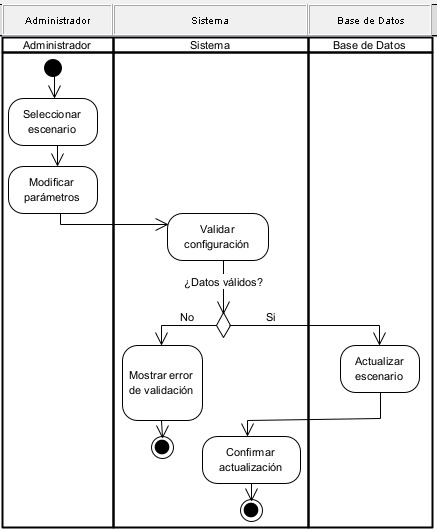
\includegraphics[width=\textwidth,height=0.85\textheight,keepaspectratio]{Actividad/actividad7.jpeg}
	\caption{Diagrama de Actividad – Configuración de Escenarios. Este diagrama muestra el flujo de configuración de escenarios realizado por el administrador.}
\end{figure}

% =====================================================
\subsubsection*{DA-08: Gestión de Normativas}
% =====================================================

\begin{figure}[H]
	\centering
	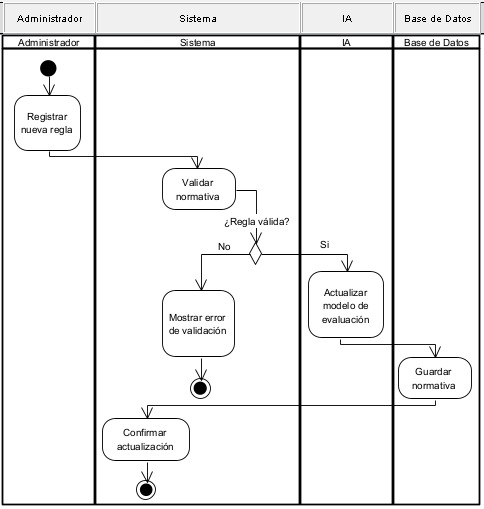
\includegraphics[width=\textwidth,height=0.85\textheight,keepaspectratio]{Actividad/actividad8.jpeg}
	\caption{Diagrama de Actividad – Gestión de Normativas. Este diagrama describe el proceso de registro y actualización de normativas dentro del sistema.}
\end{figure}

	% =====================================================
\subsection{Casos de Uso Detallado}
\subsubsection{Iniciar Sesión}

\begin{table}[H]
\centering
\resizebox{\textwidth}{!}{
\begin{tabular}{|p{3cm}|p{5.5cm}|p{5.5cm}|}
\hline
\multicolumn{1}{|c|}{\textbf{Campo}} & \multicolumn{2}{c|}{\textbf{Detalle}} \\ \hline
ID & \multicolumn{2}{p{11cm}|}{CU-01} \\ \hline
Nombre & \multicolumn{2}{p{11cm}|}{Iniciar sesión} \\ \hline
Actores & \multicolumn{2}{p{11cm}|}{Usuario} \\ \hline
Tipo & \multicolumn{2}{p{11cm}|}{Primario} \\ \hline
Descripción & \multicolumn{2}{p{11cm}|}{Permite autenticar al usuario en el sistema.} \\ \hline
Precondiciones & \multicolumn{2}{p{11cm}|}{Usuario previamente registrado.} \\ \hline
Postcondiciones & \multicolumn{2}{p{11cm}|}{Usuario autenticado y redirigido según su rol.} \\ \hline

\multirow{7}{*}{\raggedright Flujo principal}
& \textbf{Actor} & \textbf{Sistema} \\ \cline{2-3}
& 1. El caso de uso inicia cuando el usuario selecciona “Iniciar sesión”. & \\ \cline{2-3}
& & 2. El sistema muestra el formulario de autenticación. \\ \cline{2-3}
& 3. El usuario ingresa sus credenciales. & \\ \cline{2-3}
& & 4. El sistema valida las credenciales. \\ \cline{2-3}
& & 5. El sistema autentica al usuario. \\ \cline{2-3}
& & 6. El sistema redirige al entorno correspondiente. \\ \cline{2-3}
& & 7. El caso de uso finaliza cuando el usuario accede al sistema. \\ \hline

\multirow{3}{*}{\raggedright Flujo alternativo}
& \textbf{Condición / Desviación} & \textbf{Tratamiento} \\ \cline{2-3}
& 3.1 Campos vacíos. & El sistema solicita completar los datos y retorna al paso 3. \\ \cline{2-3}
& 4.1 Credenciales incorrectas. & El sistema muestra mensaje de error y retorna al paso 3. \\ \cline{2-3}
& 4.2 Error interno durante la validación. & El sistema informa la situación y termina el caso de uso. \\ \hline

Requisitos & \multicolumn{2}{p{11cm}|}{RF-01, RNF-03} \\ \hline
\end{tabular}
}
\end{table}

\subsubsection{Seleccionar Escenario de Conducción}

\begin{table}[H]
\centering
\resizebox{\textwidth}{!}{
\begin{tabular}{|p{3cm}|p{5.2cm}|p{5.5cm}|}
\hline
\multicolumn{1}{|c|}{\textbf{Campo}} & \multicolumn{2}{c|}{\textbf{Detalle}} \\ \hline
ID & \multicolumn{2}{p{11cm}|}{CU-02} \\ \hline
Nombre & \multicolumn{2}{p{11cm}|}{Seleccionar escenario de conducción} \\ \hline
Actores & \multicolumn{2}{p{11cm}|}{Usuario} \\ \hline
Tipo & \multicolumn{2}{p{11cm}|}{Primario} \\ \hline
Descripción & \multicolumn{2}{p{11cm}|}{Permite al usuario elegir el entorno de práctica y configurar la dificultad.} \\ \hline
Precondiciones & \multicolumn{2}{p{11cm}|}{Usuario autenticado.} \\ \hline
Postcondiciones & \multicolumn{2}{p{11cm}|}{Escenario configurado y listo para iniciar la práctica.} \\ \hline

\multirow{7}{*}{\raggedright Flujo principal}
& \textbf{Actor} & \textbf{Sistema} \\ \cline{2-3}
& 1. El caso de uso inicia cuando el usuario selecciona “Escenarios”. & \\ \cline{2-3}
& & 2. El sistema muestra el catálogo disponible. \\ \cline{2-3}
& 3. El usuario selecciona un escenario. & \\ \cline{2-3}
& & 4. El sistema solicita configuración de dificultad. \\ \cline{2-3}
& 5. El usuario define la dificultad. & \\ \cline{2-3}
& & 6. El sistema confirma la selección y prepara el entorno. \\ \cline{2-3}
& & 7. El caso de uso finaliza cuando el escenario queda listo. \\ \hline

\multirow{3}{*}{\raggedright Flujo alternativo}
& \textbf{Condición / Desviación} & \textbf{Tratamiento} \\ \cline{2-3}
& 2.1 No existen escenarios disponibles. & El sistema informa la situación y termina el caso de uso. \\ \cline{2-3}
& 3.1 Escenario no disponible temporalmente. & El sistema notifica y retorna al paso 2. \\ \cline{2-3}
& 5.1 Configuración inválida. & El sistema solicita corrección y retorna al paso 5. \\ \hline

Requisitos & \multicolumn{2}{p{11cm}|}{RF-02, RF-03} \\ \hline
\end{tabular}
}
\end{table}

\subsubsection{Realizar Práctica de Conducción}

\begin{table}[H]
\centering
\resizebox{\textwidth}{!}{
\begin{tabular}{|p{3cm}|p{5.5cm}|p{5.5cm}|}
\hline
\multicolumn{1}{|c|}{\textbf{Campo}} & \multicolumn{2}{c|}{\textbf{Detalle}} \\ \hline
ID & \multicolumn{2}{p{11cm}|}{CU-03} \\ \hline
Nombre & \multicolumn{2}{p{11cm}|}{Realizar práctica de conducción} \\ \hline
Actores & \multicolumn{2}{p{11cm}|}{Usuario} \\ \hline
Tipo & \multicolumn{2}{p{11cm}|}{Primario} \\ \hline
Descripción & \multicolumn{2}{p{11cm}|}{Permite ejecutar la simulación y registrar decisiones del usuario.} \\ \hline
Precondiciones & \multicolumn{2}{p{11cm}|}{Escenario previamente configurado.} \\ \hline
Postcondiciones & \multicolumn{2}{p{11cm}|}{Sesión registrada para análisis posterior.} \\ \hline

\multirow{8}{*}{\raggedright Flujo principal}
& \textbf{Actor} & \textbf{Sistema} \\ \cline{2-3}
& 1. El caso de uso inicia cuando el usuario presiona “Iniciar práctica”. & \\ \cline{2-3}
& & 2. El sistema carga el entorno de simulación. \\ \cline{2-3}
& 3. El usuario interactúa con los controles. & \\ \cline{2-3}
& & 4. El sistema procesa acciones en tiempo real. \\ \cline{2-3}
& & 5. El sistema evalúa el desempeño. \\ \cline{2-3}
& 6. El usuario finaliza la práctica. & \\ \cline{2-3}
& & 7. El sistema guarda los resultados. \\ \cline{2-3}
& & 8. El caso de uso finaliza cuando se confirma el registro. \\ \hline

\multirow{3}{*}{\raggedright Flujo alternativo}
& \textbf{Condición / Desviación} & \textbf{Tratamiento} \\ \cline{2-3}
& 2.1 Error al cargar entorno. & El sistema informa el error y termina el caso de uso. \\ \cline{2-3}
& 4.1 Fallo técnico durante la simulación. & El sistema guarda progreso y termina el caso de uso. \\ \cline{2-3}
& 6.1 El usuario abandona antes de finalizar. & El sistema guarda estado parcial y termina el caso de uso. \\ \hline

Requisitos & \multicolumn{2}{p{11cm}|}{RF-03, RF-04, RNF-01} \\ \hline
\end{tabular}
}
\end{table}
\subsubsection{Recibir Retroalimentación Automática}

\begin{table}[H]
\centering
\resizebox{\textwidth}{!}{
\begin{tabular}{|p{3cm}|p{5.5cm}|p{5.5cm}|}
\hline
\multicolumn{1}{|c|}{\textbf{Campo}} & \multicolumn{2}{c|}{\textbf{Detalle}} \\ \hline
ID & \multicolumn{2}{p{11cm}|}{CU-04} \\ \hline
Nombre & \multicolumn{2}{p{11cm}|}{Recibir retroalimentación automática} \\ \hline
Actores & \multicolumn{2}{p{11cm}|}{Usuario} \\ \hline
Tipo & \multicolumn{2}{p{11cm}|}{Primario} \\ \hline
Descripción & \multicolumn{2}{p{11cm}|}{Genera un informe de desempeño mediante el módulo de IA.} \\ \hline
Precondiciones & \multicolumn{2}{p{11cm}|}{Práctica finalizada y registrada.} \\ \hline
Postcondiciones & \multicolumn{2}{p{11cm}|}{Informe visualizado o almacenado para consulta posterior.} \\ \hline

\multirow{7}{*}{\raggedright Flujo principal}
& \textbf{Actor} & \textbf{Sistema} \\ \cline{2-3}
& 1. El caso de uso inicia cuando el usuario selecciona “Ver retroalimentación”. & \\ \cline{2-3}
& & 2. El sistema envía los datos al módulo IA. \\ \cline{2-3}
& & 3. La IA analiza el desempeño. \\ \cline{2-3}
& & 4. El sistema genera el informe. \\ \cline{2-3}
& & 5. El sistema muestra los resultados al usuario. \\ \cline{2-3}
& & 6. El sistema almacena el informe. \\ \cline{2-3}
& & 7. El caso de uso finaliza cuando el usuario visualiza el informe. \\ \hline

\multirow{3}{*}{\raggedright Flujo alternativo}
& \textbf{Condición / Desviación} & \textbf{Tratamiento} \\ \cline{2-3}
& 2.1 Error en envío de datos a IA. & El sistema informa el problema y termina el caso de uso. \\ \cline{2-3}
& 3.1 Fallo en el análisis de IA. & El sistema notifica la incidencia y termina el caso de uso. \\ \cline{2-3}
& 5.1 El usuario decide cerrar el informe. & El sistema guarda el informe y termina el caso de uso. \\ \hline

Requisitos & \multicolumn{2}{p{11cm}|}{RF-05, RF-07} \\ \hline
\end{tabular}
}
\end{table}

\subsubsection{Consultar Puntuación y Métricas}

\begin{table}[H]
\centering
\resizebox{\textwidth}{!}{
\begin{tabular}{|p{3cm}|p{5.5cm}|p{5.5cm}|}
\hline
\multicolumn{1}{|c|}{\textbf{Campo}} & \multicolumn{2}{c|}{\textbf{Detalle}} \\ \hline
ID & \multicolumn{2}{p{11cm}|}{CU-05} \\ \hline
Nombre & \multicolumn{2}{p{11cm}|}{Consultar puntuación y métricas} \\ \hline
Actores & \multicolumn{2}{p{11cm}|}{Usuario} \\ \hline
Tipo & \multicolumn{2}{p{11cm}|}{Secundario} \\ \hline
Descripción & \multicolumn{2}{p{11cm}|}{Permite visualizar el historial de desempeño acumulado.} \\ \hline
Precondiciones & \multicolumn{2}{p{11cm}|}{Existencia de registros previos.} \\ \hline
Postcondiciones & \multicolumn{2}{p{11cm}|}{Reporte visualizado correctamente.} \\ \hline

\multirow{7}{*}{\raggedright Flujo principal}
& \textbf{Actor} & \textbf{Sistema} \\ \cline{2-3}
& 1. El caso de uso inicia cuando el usuario selecciona “Mis estadísticas”. & \\ \cline{2-3}
& & 2. El sistema recupera el historial del usuario. \\ \cline{2-3}
& & 3. El sistema calcula métricas comparativas. \\ \cline{2-3}
& & 4. El sistema genera gráficos y reportes. \\ \cline{2-3}
& & 5. El sistema muestra la información. \\ \cline{2-3}
& & 6. El sistema permite opciones adicionales. \\ \cline{2-3}
& & 7. El caso de uso finaliza cuando el usuario revisa la información. \\ \hline

\multirow{3}{*}{\raggedright Flujo alternativo}
& \textbf{Condición / Desviación} & \textbf{Tratamiento} \\ \cline{2-3}
& 2.1 No existen registros previos. & El sistema informa la ausencia de datos y termina el caso de uso. \\ \cline{2-3}
& 6.1 Solicitud de exportación. & El sistema genera el archivo y retorna al paso 6. \\ \cline{2-3}
& 4.1 Error en generación de gráficos. & El sistema notifica la falla y termina el caso de uso. \\ \hline

Requisitos & \multicolumn{2}{p{11cm}|}{RF-06, RF-08, RF-09} \\ \hline
\end{tabular}
}
\end{table}

\subsubsection{Recibir Recompensas}

\begin{table}[H]
\centering
\resizebox{\textwidth}{!}{
\begin{tabular}{|p{3cm}|p{5.5cm}|p{5.5cm}|}
\hline
\multicolumn{1}{|c|}{\textbf{Campo}} & \multicolumn{2}{c|}{\textbf{Detalle}} \\ \hline
ID & \multicolumn{2}{p{11cm}|}{CU-06} \\ \hline
Nombre & \multicolumn{2}{p{11cm}|}{Recibir recompensas} \\ \hline
Actores & \multicolumn{2}{p{11cm}|}{Usuario} \\ \hline
Tipo & \multicolumn{2}{p{11cm}|}{Secundario} \\ \hline
Descripción & \multicolumn{2}{p{11cm}|}{Asigna insignias según el cumplimiento de metas.} \\ \hline
Precondiciones & \multicolumn{2}{p{11cm}|}{Cumplimiento de hitos definidos.} \\ \hline
Postcondiciones & \multicolumn{2}{p{11cm}|}{Insignia registrada en el perfil del usuario.} \\ \hline

\multirow{6}{*}{\raggedright Flujo principal}
& \textbf{Actor} & \textbf{Sistema} \\ \cline{2-3}
& 1. El caso de uso inicia cuando el usuario completa un hito. & \\ \cline{2-3}
& & 2. El sistema valida el cumplimiento. \\ \cline{2-3}
& & 3. El sistema asigna la insignia correspondiente. \\ \cline{2-3}
& & 4. El sistema actualiza el perfil. \\ \cline{2-3}
& & 5. El sistema notifica al usuario. \\ \cline{2-3}
& & 6. El caso de uso finaliza con la notificación mostrada. \\ \hline

\multirow{2}{*}{\raggedright Flujo alternativo}
& \textbf{Condición / Desviación} & \textbf{Tratamiento} \\ \cline{2-3}
& 2.1 No se cumple el hito completamente. & El sistema no asigna recompensa y termina el caso de uso. \\ \cline{2-3}
& 3.1 Error en asignación. & El sistema registra la incidencia y termina el caso de uso. \\ \hline

Requisitos & \multicolumn{2}{p{11cm}|}{RF-06} \\ \hline
\end{tabular}
}
\end{table}

\subsubsection{Configurar Escenarios}

\begin{table}[H]
\centering
\resizebox{\textwidth}{!}{
\begin{tabular}{|p{3cm}|p{5.5cm}|p{5.5cm}|}
\hline
\multicolumn{1}{|c|}{\textbf{Campo}} & \multicolumn{2}{c|}{\textbf{Detalle}} \\ \hline
ID & \multicolumn{2}{p{11cm}|}{CU-07} \\ \hline
Nombre & \multicolumn{2}{p{11cm}|}{Configurar escenarios} \\ \hline
Actores & \multicolumn{2}{p{11cm}|}{Administrador} \\ \hline
Tipo & \multicolumn{2}{p{11cm}|}{Administrativo} \\ \hline
Descripción & \multicolumn{2}{p{11cm}|}{Permite modificar parámetros de tráfico y clima.} \\ \hline
Precondiciones & \multicolumn{2}{p{11cm}|}{Administrador autenticado.} \\ \hline
Postcondiciones & \multicolumn{2}{p{11cm}|}{Parámetros actualizados correctamente.} \\ \hline

\multirow{7}{*}{\raggedright Flujo principal}
& \textbf{Actor} & \textbf{Sistema} \\ \cline{2-3}
& 1. El caso de uso inicia cuando el administrador accede al módulo de escenarios. & \\ \cline{2-3}
& & 2. El sistema muestra los escenarios configurables. \\ \cline{2-3}
& 3. El administrador selecciona uno. & \\ \cline{2-3}
& & 4. El sistema permite modificar parámetros. \\ \cline{2-3}
& 5. El administrador guarda cambios. & \\ \cline{2-3}
& & 6. El sistema valida y aplica cambios. \\ \cline{2-3}
& & 7. El caso de uso finaliza con la confirmación. \\ \hline

\multirow{2}{*}{\raggedright Flujo alternativo}
& \textbf{Condición / Desviación} & \textbf{Tratamiento} \\ \cline{2-3}
& 4.1 Parámetros inválidos. & El sistema solicita corrección y retorna al paso 4. \\ \cline{2-3}
& 6.1 Error al aplicar cambios. & El sistema informa la falla y termina el caso de uso. \\ \hline

Requisitos & \multicolumn{2}{p{11cm}|}{RF-10, RF-02} \\ \hline
\end{tabular}
}
\end{table}

\subsubsection{Actualizar Reglas de Tránsito}

\begin{table}[H]
\centering
\resizebox{\textwidth}{!}{
\begin{tabular}{|p{3cm}|p{5.5cm}|p{5.5cm}|}
\hline
\multicolumn{1}{|c|}{\textbf{Campo}} & \multicolumn{2}{c|}{\textbf{Detalle}} \\ \hline
ID & \multicolumn{2}{p{11cm}|}{CU-08} \\ \hline
Nombre & \multicolumn{2}{p{11cm}|}{Actualizar reglas de tránsito} \\ \hline
Actores & \multicolumn{2}{p{11cm}|}{Administrador} \\ \hline
Tipo & \multicolumn{2}{p{11cm}|}{Administrativo} \\ \hline
Descripción & \multicolumn{2}{p{11cm}|}{Permite registrar nuevas normativas para el motor de evaluación.} \\ \hline
Precondiciones & \multicolumn{2}{p{11cm}|}{Administrador autenticado.} \\ \hline
Postcondiciones & \multicolumn{2}{p{11cm}|}{Motor de evaluación actualizado.} \\ \hline

\multirow{7}{*}{\raggedright Flujo principal}
& \textbf{Actor} & \textbf{Sistema} \\ \cline{2-3}
& 1. El caso de uso inicia cuando el administrador accede al módulo de reglas. & \\ \cline{2-3}
& & 2. El sistema muestra las normativas actuales. \\ \cline{2-3}
& 3. El administrador registra nueva normativa. & \\ \cline{2-3}
& & 4. El sistema valida coherencia. \\ \cline{2-3}
& & 5. El sistema integra la regla al motor de evaluación. \\ \cline{2-3}
& & 6. El sistema confirma la actualización. \\ \cline{2-3}
& & 7. El caso de uso finaliza con la confirmación. \\ \hline

\multirow{2}{*}{\raggedright Flujo alternativo}
& \textbf{Condición / Desviación} & \textbf{Tratamiento} \\ \cline{2-3}
& 4.1 Conflicto entre reglas. & El sistema solicita revisión y retorna al paso 3. \\ \cline{2-3}
& 5.1 Error al integrar la regla. & El sistema informa la incidencia y termina el caso de uso. \\ \hline

Requisitos & \multicolumn{2}{p{11cm}|}{RF-10, RF-05} \\ \hline
\end{tabular}
}
\end{table}
	% =====================================================
	\section{Escenarios del Sistema}
	% =====================================================
	
	% =====================================================
	\subsection{Escenario 1: Conducción Normal}
	% =====================================================
	
	\begin{longtable}{|p{4cm}|p{10cm}|}
		\hline
		\textbf{Campo} & \textbf{Detalle} \\ \hline
		
		ID / Nombre & ESC-01: Conducción Normal \\ \hline
		
		Descripción &
		El conductor interactúa con el simulador respetando las señales de tránsito, manteniendo la velocidad adecuada y respondiendo correctamente ante peatones y otros vehículos. \\ \hline
		
		Precondiciones &
		1) Sesión iniciada correctamente. \newline
		2) Escenario cargado en el entorno. \newline
		3) Sensores de IA activos para monitoreo del comportamiento. \\ \hline
		
		Secuencia de Pasos &
		1) El conductor inicia la marcha observando la señalética representada por el sistema. \newline
		2) El sistema simula dinámicamente peatones y otros vehículos. \newline
		3) El conductor toma decisiones (frenar, girar, acelerar) respetando la normativa. \newline
		4) La IA evalúa las acciones en tiempo real. \\ \hline
		
		Resultado Esperado &
		El sistema registra un desempeño positivo y genera retroalimentación favorable para el usuario. \\ \hline
		
		Requisitos Relacionados &
		RF-03, RF-04, RF-05 \\ \hline
		
	\end{longtable}
	
	% =====================================================
	\subsection{Escenario 2: Infracción de Tránsito}
	% =====================================================
	
	\begin{longtable}{|p{4cm}|p{10cm}|}
		\hline
		\textbf{Campo} & \textbf{Detalle} \\ \hline
		
		ID / Nombre & ESC-02: Infracción de Tránsito \\ \hline
		
		Descripción &
		El conductor realiza una acción indebida, como exceder el límite de velocidad o ignorar una señal durante la práctica. \\ \hline
		
		Precondiciones &
		1) Simulación en curso. \newline
		2) Módulo de IA conectado a la base de datos de normativas vigentes. \\ \hline
		
		Secuencia de Pasos &
		1) El conductor excede el límite de velocidad o ignora una señal de tránsito. \newline
		2) El sistema detecta la infracción mediante el análisis del módulo de IA. \newline
		3) El sistema actualiza las métricas de desempeño del usuario en tiempo real. \newline
		4) El evento queda registrado en el historial de la base de datos. \\ \hline
		
		Resultado Esperado &
		La infracción es detectada, documentada y afecta la puntuación de seguridad vial del conductor. \\ \hline
		
		Requisitos Relacionados &
		RF-05, RF-06, RF-08 \\ \hline
		
	\end{longtable}
	
	% =====================================================
	\subsection{Escenario 3: Evaluación Final}
	% =====================================================
	
	\begin{longtable}{|p{4cm}|p{10cm}|}
		\hline
		\textbf{Campo} & \textbf{Detalle} \\ \hline
		
		ID / Nombre & ESC-03: Evaluación Final \\ \hline
		
		Descripción &
		Al finalizar la simulación, el sistema consolida y procesa todas las métricas registradas durante la práctica. \\ \hline
		
		Precondiciones &
		1) Práctica de conducción finalizada correctamente. \newline
		2) Datos de la sesión almacenados en la Base de Datos. \\ \hline
		
		Secuencia de Pasos &
		1) El sistema recupera el historial de movimientos y decisiones de la sesión actual. \newline
		2) El módulo de IA genera un diagnóstico pedagógico basado en aciertos y errores. \newline
		3) El sistema genera un reporte de desempeño detallado. \newline
		4) El usuario visualiza la retroalimentación personalizada en pantalla. \\ \hline
		
		Resultado Esperado &
		Se genera un informe que permite al usuario comprender sus fallos y recibir recomendaciones educativas personalizadas. \\ \hline
		
		Requisitos Relacionados &
		RF-07, RF-09 \\ \hline
		
	\end{longtable}
	
	
	
	\subsection{Diagrama de Clases}
	
	Este diagrama está compuesto por diversas clases que representan los actores, componentes funcionales y módulos de análisis. A continuación se describen las clases, sus atributos, métodos y relaciones:
	
	\subsubsection*{Clase \texttt{Usuario}}
	Representa al participante del simulador.
	
	\begin{itemize}
		\item \textbf{Atributos:}
		\begin{itemize}
			\item \texttt{idUsuario}: Identificador único del usuario.
			\item \texttt{nombre}: Nombre del usuario.
			\item \texttt{rol}: Tipo de usuario (por ejemplo, aprendiz).
			\item \texttt{historialPractica}: Registro de prácticas realizadas.
		\end{itemize}
		\item \textbf{Métodos:}
		\begin{itemize}
			\item \texttt{iniciarSesion()}
			\item \texttt{seleccionarEscenario()}
			\item \texttt{realizarPractica()}
			\item \texttt{consultarResultado()}
		\end{itemize}
	\end{itemize}
	
	\subsubsection*{Clase \texttt{Administrador}}
	Encargado de la configuración y gestión del sistema.
	
	\begin{itemize}
		\item \textbf{Atributos:}
		\begin{itemize}
			\item \texttt{credenciales}: Datos de acceso del administrador.
		\end{itemize}
		\item \textbf{Métodos:}
		\begin{itemize}
			\item \texttt{configurarEscenario()}
			\item \texttt{gestionarUsuario()}
			\item \texttt{actualizarReglasTransito()}
		\end{itemize}
	\end{itemize}
	
	\subsubsection*{Clase \texttt{Simulador}}
	Controla el flujo de la simulación.
	
	\begin{itemize}
		\item \textbf{Atributos:}
		\begin{itemize}
			\item \texttt{escenarioActual}: Escenario en ejecución.
			\item \texttt{estadoSimulacion}: Estado actual del simulador.
		\end{itemize}
		\item \textbf{Métodos:}
		\begin{itemize}
			\item \texttt{iniciarSimulacion()}
			\item \texttt{finalizarSimulacion()}
			\item \texttt{registrarDecision(usuario, decision)}
			\item \texttt{generarRetroalimentacion()}
		\end{itemize}
	\end{itemize}
	
	\subsubsection*{Clase \texttt{Escenario}}
	Define el entorno de simulación.
	
	\begin{itemize}
		\item \textbf{Atributos:}
		\begin{itemize}
			\item \texttt{idEscenario}: Identificador del escenario.
			\item \texttt{tipo}: Tipo de escenario (urbano, rural, etc.).
			\item \texttt{nivelDificultad}: Grado de complejidad.
		\end{itemize}
		\item \textbf{Métodos:}
		\begin{itemize}
			\item \texttt{cargarEscenario()}
			\item \texttt{validarCondiciones()}
		\end{itemize}
	\end{itemize}
	
	\subsubsection*{Clase \texttt{Métricas}}
	Evalúa el rendimiento del usuario.
	
	\begin{itemize}
		\item \textbf{Atributos:}
		\begin{itemize}
			\item \texttt{puntaje}: Calificación obtenida.
			\item \texttt{erroresCometidos}: Fallos durante la práctica.
			\item \texttt{tiempoReaccion}: Tiempo de respuesta ante eventos.
		\end{itemize}
		\item \textbf{Métodos:}
		\begin{itemize}
			\item \texttt{calcularPuntaje()}
			\item \texttt{generarReporte()}
			\item \texttt{compararHistorial()}
		\end{itemize}
	\end{itemize}
	
	\subsubsection*{Clase \texttt{Recompensa}}
	Entrega incentivos al usuario.
	
	\begin{itemize}
		\item \textbf{Atributos:}
		\begin{itemize}
			\item \texttt{nivel}: Nivel alcanzado.
			\item \texttt{insignias}: Distinciones obtenidas.
		\end{itemize}
		\item \textbf{Métodos:}
		\begin{itemize}
			\item \texttt{asignarRecompensa()}
			\item \texttt{mostrarRecompensas()}
		\end{itemize}
	\end{itemize}
	
	\subsubsection*{Clase \texttt{IA}}
	Módulo de inteligencia artificial para análisis predictivo.
	
	\begin{itemize}
		\item \textbf{Atributos:}
		\begin{itemize}
			\item \texttt{modeloPredictivo}: Algoritmo utilizado.
			\item \texttt{precision}: Nivel de exactitud del modelo.
		\end{itemize}
		\item \textbf{Métodos:}
		\begin{itemize}
			\item \texttt{analizarDecision()}
			\item \texttt{evaluarComportamiento()}
			\item \texttt{generarPuntuacion()}
		\end{itemize}
	\end{itemize}
	
	\subsubsection*{Relaciones entre clases}
	\begin{itemize}
		\item \texttt{Usuario} interactúa con \texttt{Simulador}, seleccionando escenarios y realizando prácticas.
		\item \texttt{Simulador} utiliza \texttt{Escenario} para ejecutar la simulación.
		\item \texttt{Simulador} registra decisiones del \texttt{Usuario} y genera retroalimentación con ayuda de \texttt{IA}.
		\item \texttt{Métricas} evalúa el desempeño del \texttt{Usuario} y puede influir en la \texttt{Recompensa}.
		\item \texttt{Administrador} configura \texttt{Escenario} y gestiona \texttt{Usuario}.
		\item \texttt{IA} complementa el análisis de decisiones y comportamiento para enriquecer las \texttt{Métricas}.
	\end{itemize}
	
	\begin{figure}[H]
		\centering
		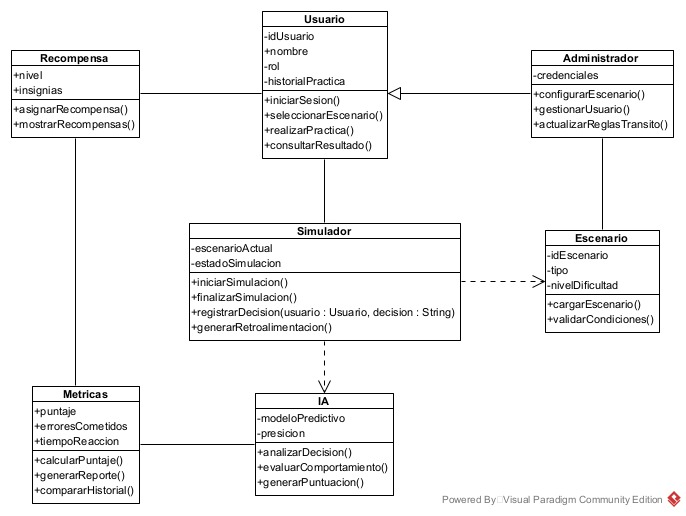
\includegraphics[width=0.9\textwidth]{Clase/Diagrama de Clases1.jpeg}
		\caption{Diagrama de Clases (nivel análisis)}
	\end{figure}
	
	% =========================
	\section{Validación y Verificación de Requisitos}
	
	La validación y verificación constituyen actividades esenciales para garantizar calidad en la Ingeniería de Requerimientos \cite{ISO29148,Khalid2025}.
	
	\subsection{Validación}
	
	La validación se realizó mediante revisión con stakeholders y contraste con metas GORE, asegurando que:
	
	\begin{itemize}
		\item Cada requisito contribuya a un objetivo identificado.
		\item Los escenarios representen situaciones reales del dominio vial.
		\item Los actores comprendan el alcance del sistema.
	\end{itemize}
	
	\subsection{Verificación}
	
	Se aplicaron criterios formales de calidad:
	
	\begin{itemize}
		\item Claridad y ausencia de ambigüedad.
		\item Consistencia entre requisitos.
		\item Posibilidad de prueba o medición.
		\item Trazabilidad hacia metas y escenarios.
	\end{itemize}
	
	
	% =========================
	\section{Trazabilidad de Requisitos}
	
	La trazabilidad permite establecer relaciones claras entre los objetivos del sistema, los escenarios y los requisitos funcionales y no funcionales, facilitando la gestión de cambios y el control del alcance \cite{Gotel1994}.
	
	La Tabla~\ref{tab:trazabilidad} presenta una matriz de trazabilidad simplificada que relaciona los objetivos principales con los requisitos identificados.
	
	\begin{table}[H]
		\centering
		\caption{Matriz de Trazabilidad Mejorada}
		\label{tab:trazabilidad}
		\begin{tabular}{p{3cm} p{3cm} p{4cm} p{3cm}}
			\toprule
			\textbf{Meta} & \textbf{Escenario} & \textbf{Requisito} & \textbf{Tipo} \\
			\midrule
			Mejorar comportamiento vial & Conducción normal & RF-05 (Análisis IA) & Funcional \\
			Evaluar decisiones & Infracción & RF-06 (Métricas) & Funcional \\
			Retroalimentación educativa & Evaluación final & RF-07 & Funcional \\
			Proteger datos & Uso del sistema & RNF-03 & No Funcional \\
			Rendimiento estable & Simulación activa & RNF-01 & No Funcional \\
			\bottomrule
		\end{tabular}
	\end{table}
	
	La tabla presenta una muestra representativa de la trazabilidad establecida; sin embargo, todos los requisitos definidos fueron vinculados internamente con sus respectivas metas y escenarios durante el proceso de validación.
	
	% =========================
	\section{Gestión de Cambios}
	
	Durante la fase de análisis se identificó la necesidad de gestionar cambios de manera controlada, considerando que los requisitos pueden evolucionar conforme se obtiene retroalimentación de los usuarios y actores involucrados \cite{Wiegers2013}.
	
	Se establece que cualquier cambio propuesto deberá:
	\begin{itemize}
		\item Ser justificado por un stakeholder.
		\item Analizar su impacto en los objetivos y requisitos existentes.
		\item Actualizar la matriz de trazabilidad.
	\end{itemize}
	
	Este enfoque reduce riesgos asociados a modificaciones no controladas del alcance.
	
	% =========================
	\section{Resultados y Discusión}
	
	El proceso de Ingeniería de Requerimientos aplicado permitió identificar de manera estructurada los objetivos, actores y requisitos del simulador vial. El uso del enfoque GORE facilitó la alineación entre las metas estratégicas y los requisitos funcionales y no funcionales definidos.
	
	Asimismo, la aplicación de técnicas de elicitación y la validación temprana contribuyeron a reducir ambigüedades y a mejorar la calidad de la especificación. A diferencia de los enfoques centrados exclusivamente en modelos predictivos, este trabajo prioriza la formalización temprana de requisitos como base para el desarrollo posterior de soluciones inteligentes \cite{Ferrari2021}.
	
	% =========================
	\newpage
	\section{Conclusiones}
	El informe parcial también permitió identificar dependencias críticas entre los objetivos del sistema y los actores involucrados, lo que facilita la trazabilidad de los requisitos en etapas posteriores. Asimismo, el análisis realizado contribuyó a detectar posibles riesgos y limitaciones, ofreciendo lineamientos iniciales para su mitigación dentro del simulador.
	
	La integración del enfoque GORE con el modelado conceptual asegura que las metas estratégicas se traduzcan en funcionalidades concretas, fortaleciendo la coherencia entre la visión del sistema y su implementación técnica. De esta manera, se establece un marco metodológico que no solo respalda la validez académica del proyecto, sino que también garantiza su aplicabilidad práctica en escenarios de simulación de tránsito.
	
	En conjunto, estos avances consolidan una base robusta para la siguiente fase de especificación detallada, donde se profundizará en los casos de uso, métricas de evaluación y mecanismos de retroalimentación que permitirán validar el desempeño del simulador frente a los objetivos planteados.
	
	\newpage
	\section{Referencias}
	\printbibliography
	
	\newpage
	\section{Anexos}
	\subsection{Capturas de Pantalla}
	
	% --------- CAPTURAS 1 y 2 ----------
	\begin{figure}[H]
		\centering
		\begin{minipage}{0.45\textwidth}
			\centering
			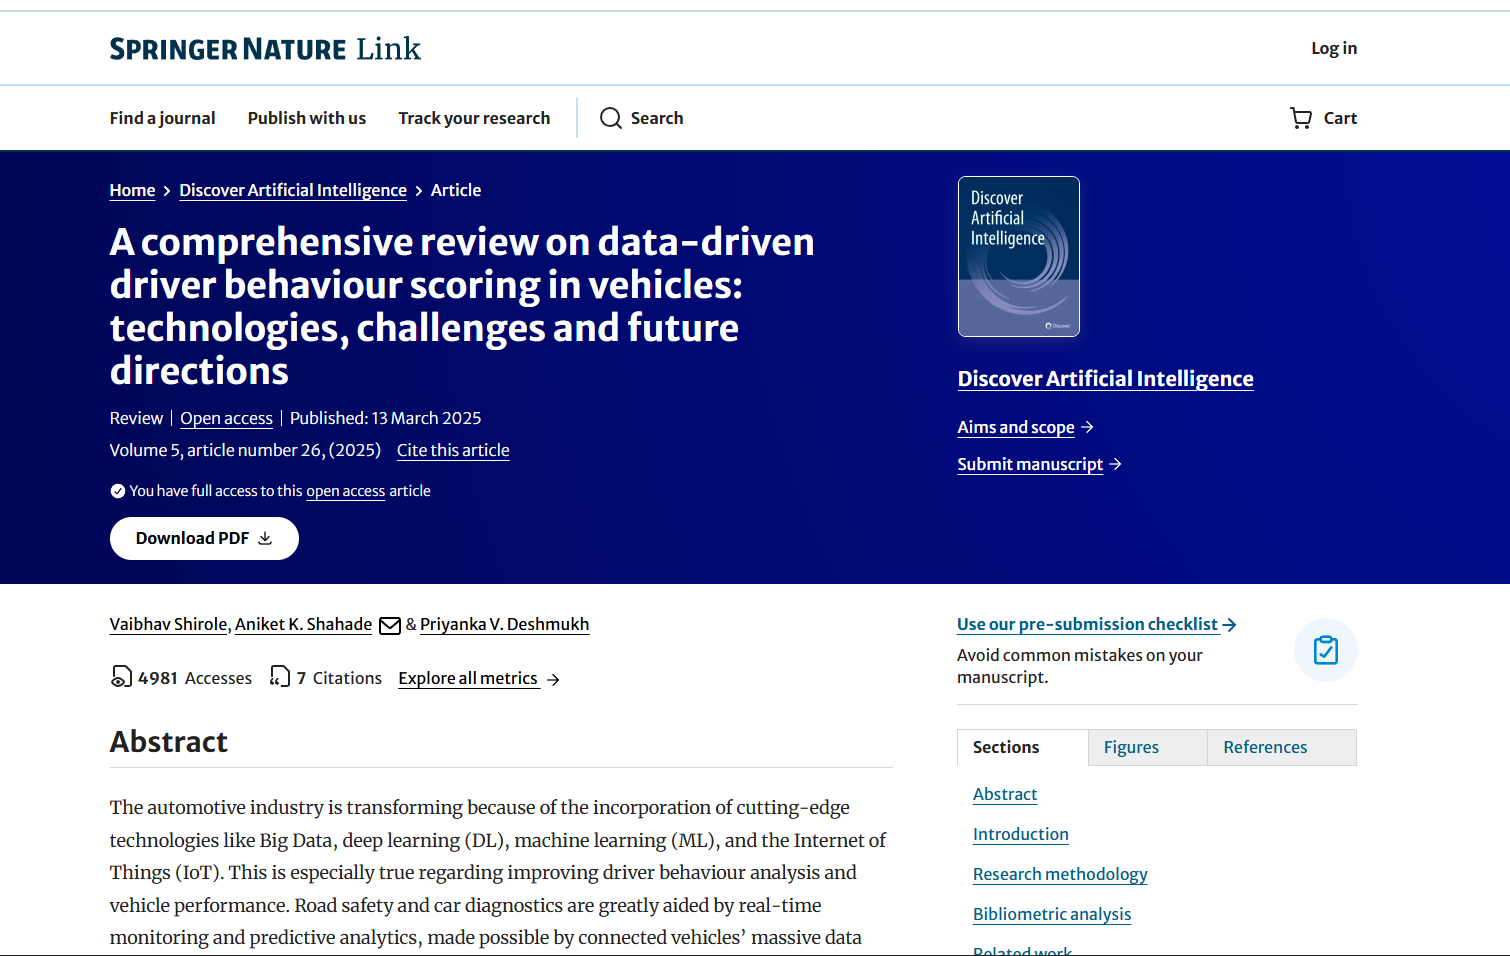
\includegraphics[width=\linewidth]{Anexo/Captura 1.png}
			\caption{A comprehensive review on data-driven driver behaviour scoring in vehicles}
		\end{minipage}\hfill
		\begin{minipage}{0.45\textwidth}
			\centering
			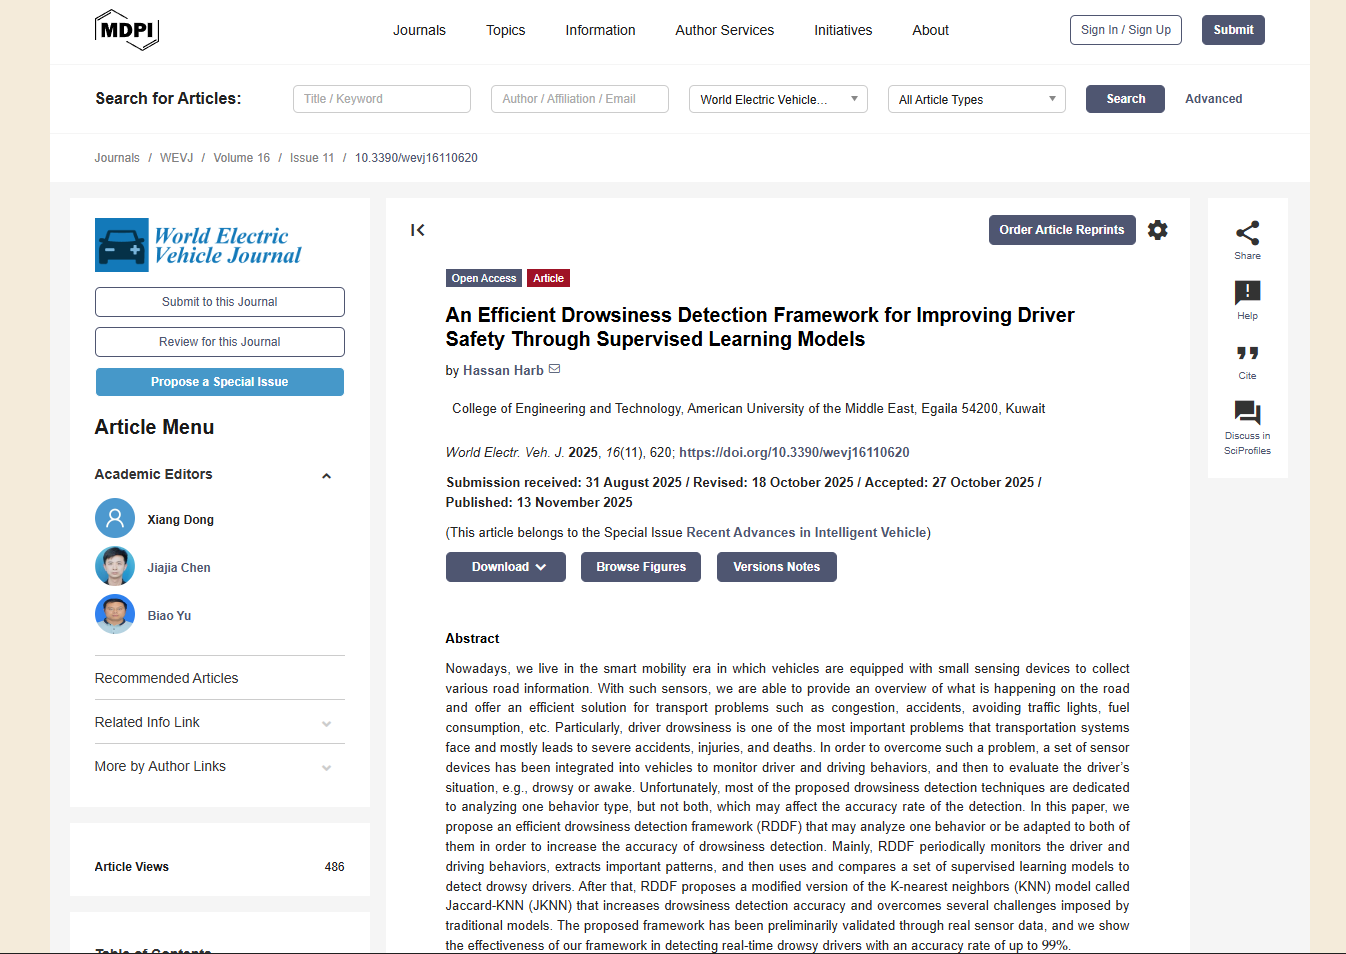
\includegraphics[width=\linewidth]{Anexo/Captura 2.png}
			\caption{An Efficient Drowsiness Detection Framework}
		\end{minipage}
	\end{figure}
	
	% --------- CAPTURAS 3 y 4 ----------
	\begin{figure}[H]
		\centering
		\begin{minipage}{0.45\textwidth}
			\centering
			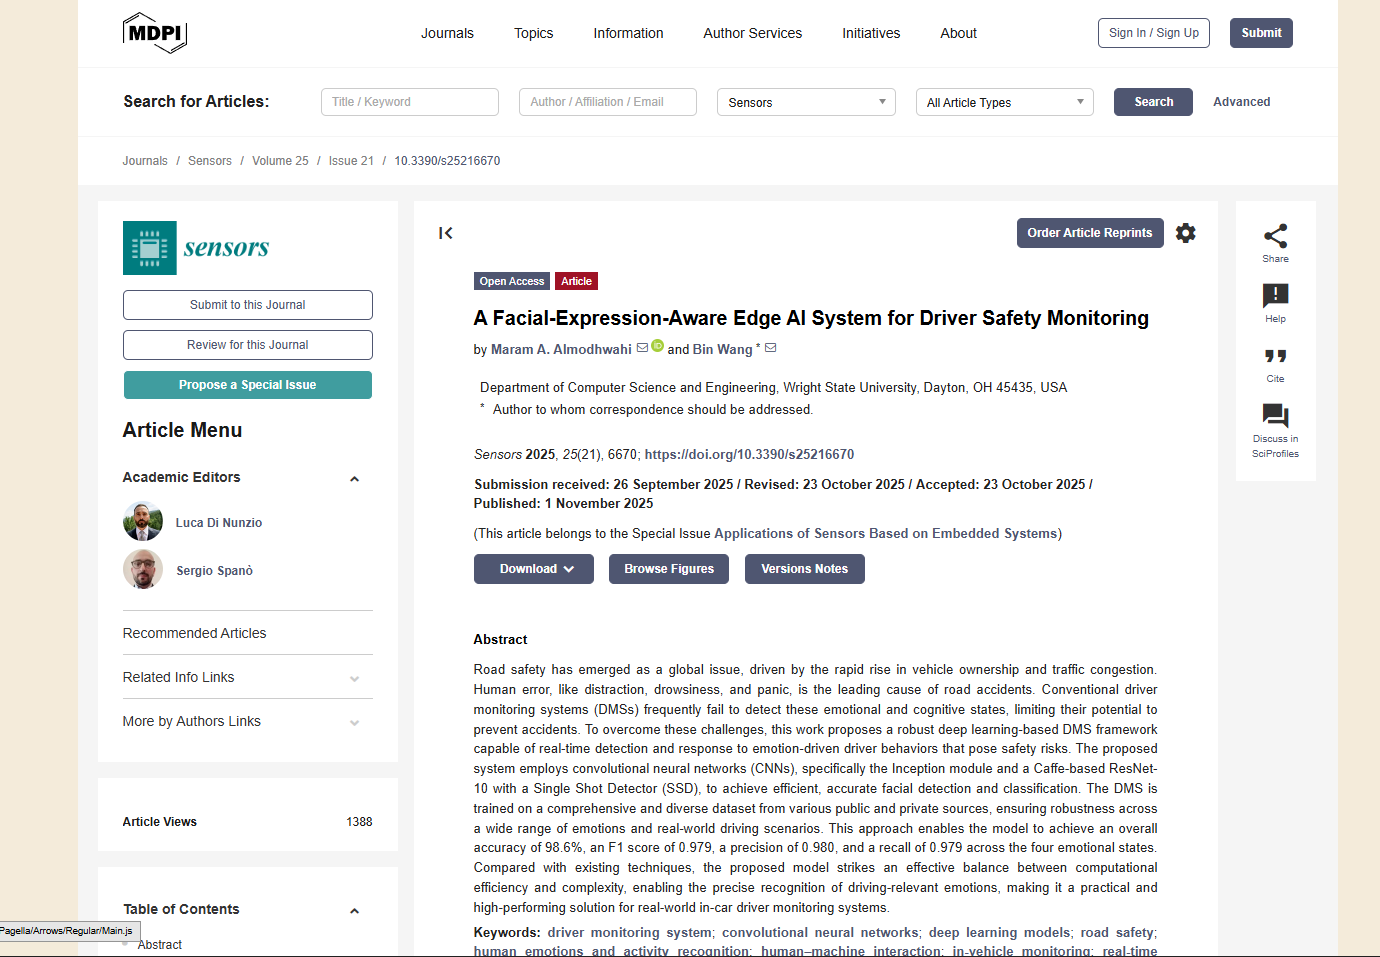
\includegraphics[width=\linewidth]{Anexo/Captura 3.png}
			\caption{A Facial-Expression-Aware Edge AI System}
		\end{minipage}\hfill
		\begin{minipage}{0.45\textwidth}
			\centering
			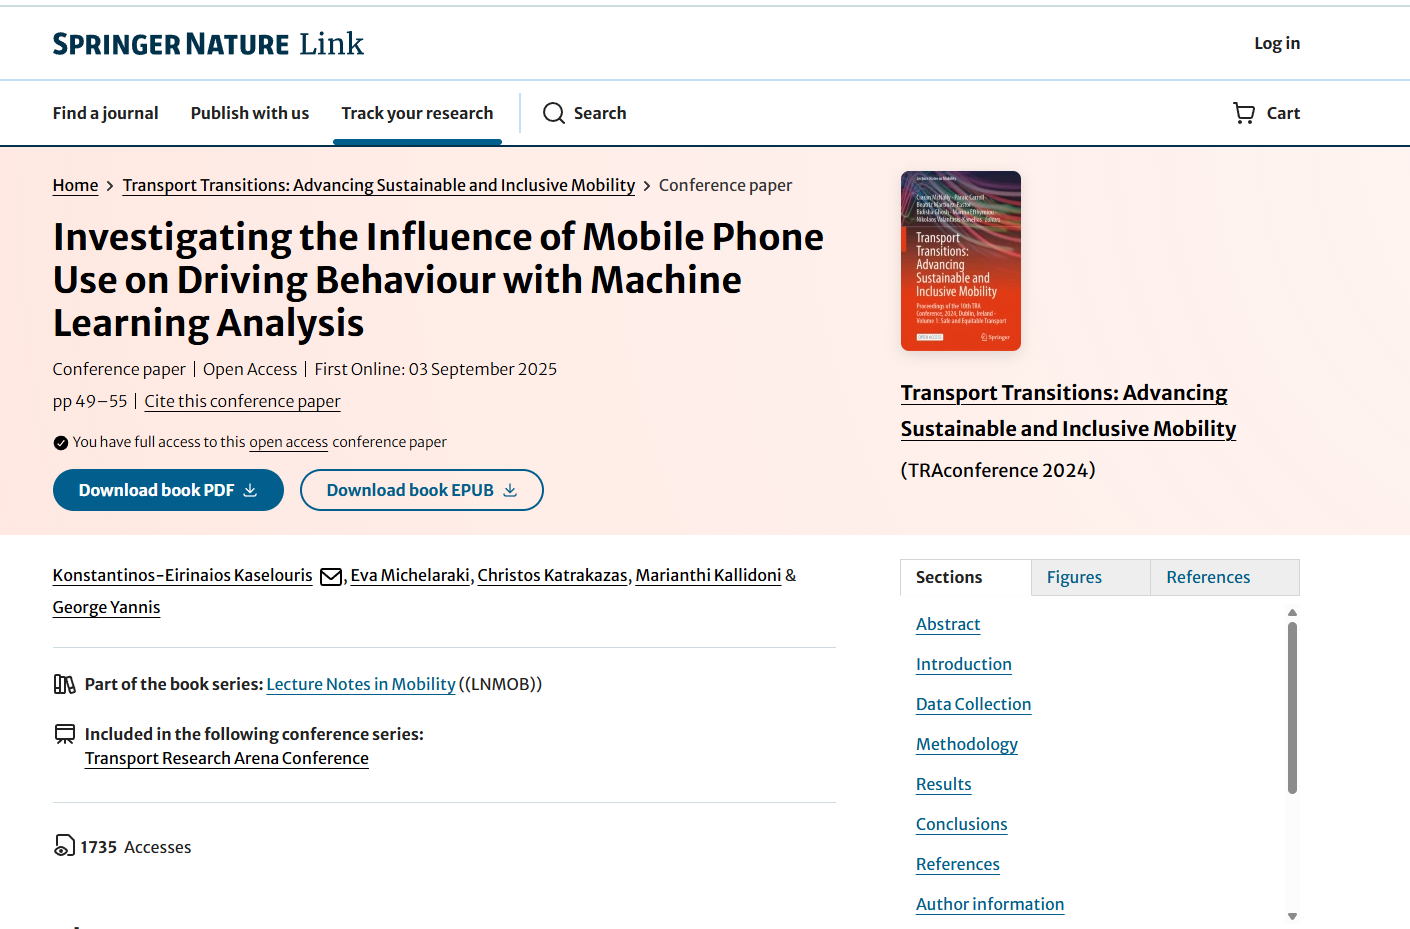
\includegraphics[width=\linewidth]{Anexo/Captura 4.png}
			\caption{Investigating the Influence of Mobile Phone Use on Driving Behaviour}
		\end{minipage}
	\end{figure}
	
	\newpage
	
	% --------- CAPTURAS 5 y 6 ----------
	\begin{figure}[H]
		\centering
		\begin{minipage}{0.45\textwidth}
			\centering
			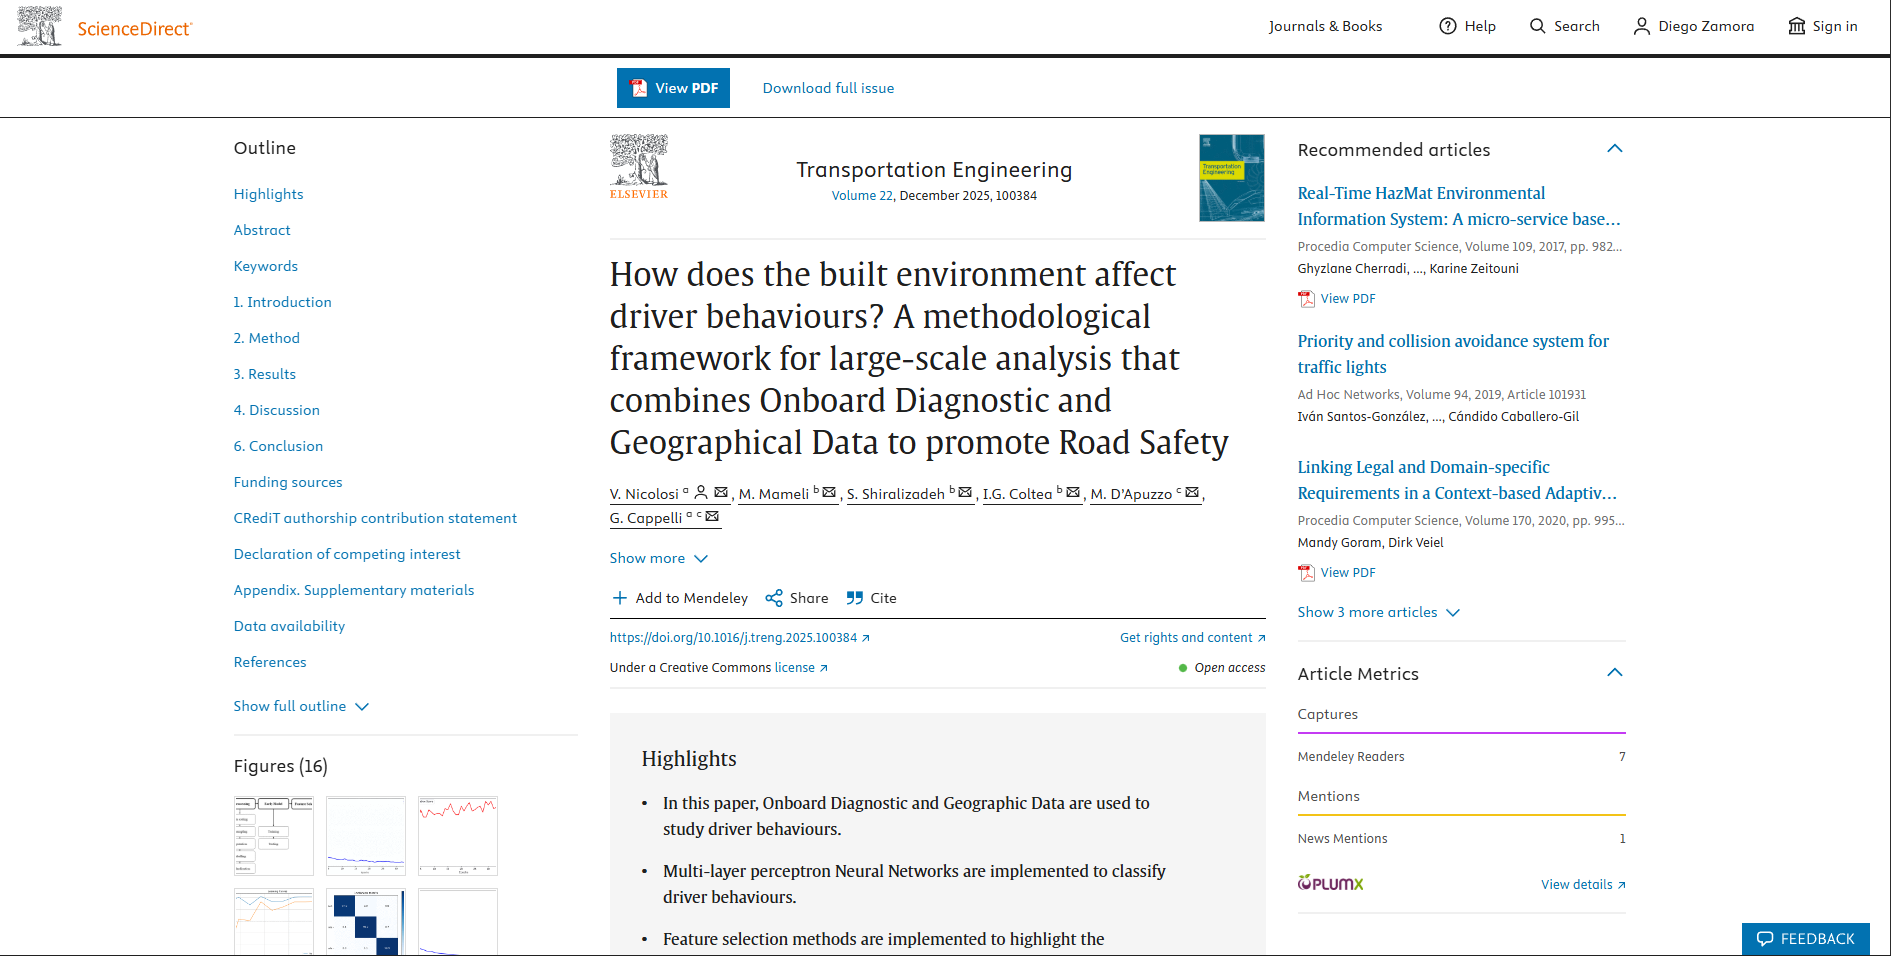
\includegraphics[width=\linewidth]{Anexo/Captura 5.png}
			\caption{How does the built environment affect driver behaviours? A methodological framework for large-scale analysis that combines Onboard Diagnostic and Geographical Data to promote Road Safety}
		\end{minipage}\hfill
		\begin{minipage}{0.45\textwidth}
			\centering
			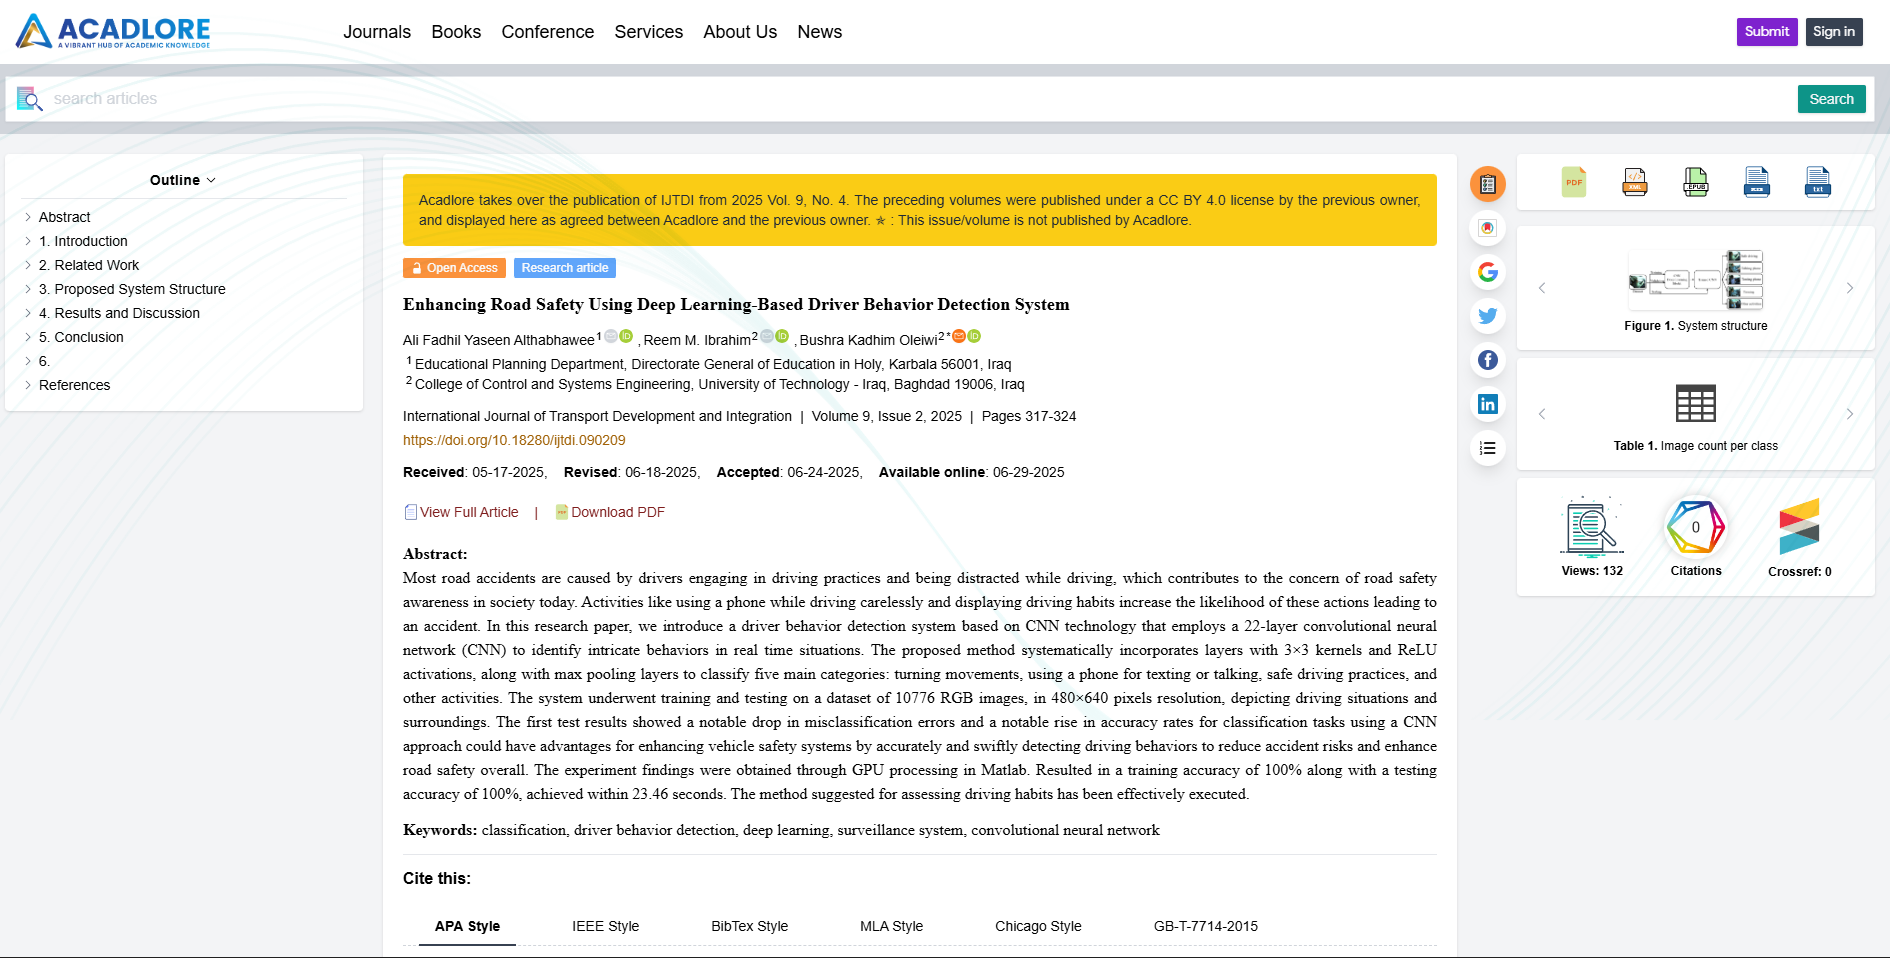
\includegraphics[width=\linewidth]{Anexo/Captura 6.png}
			\caption{An Efficient Drowsiness Detection Framework}
		\end{minipage}
	\end{figure}
	
	% --------- CAPTURA 7 (IZQUIERDA, MISMO TAMAÑO) ----------
	\begin{figure}[H]
		\raggedright
		\begin{minipage}{0.45\textwidth}
			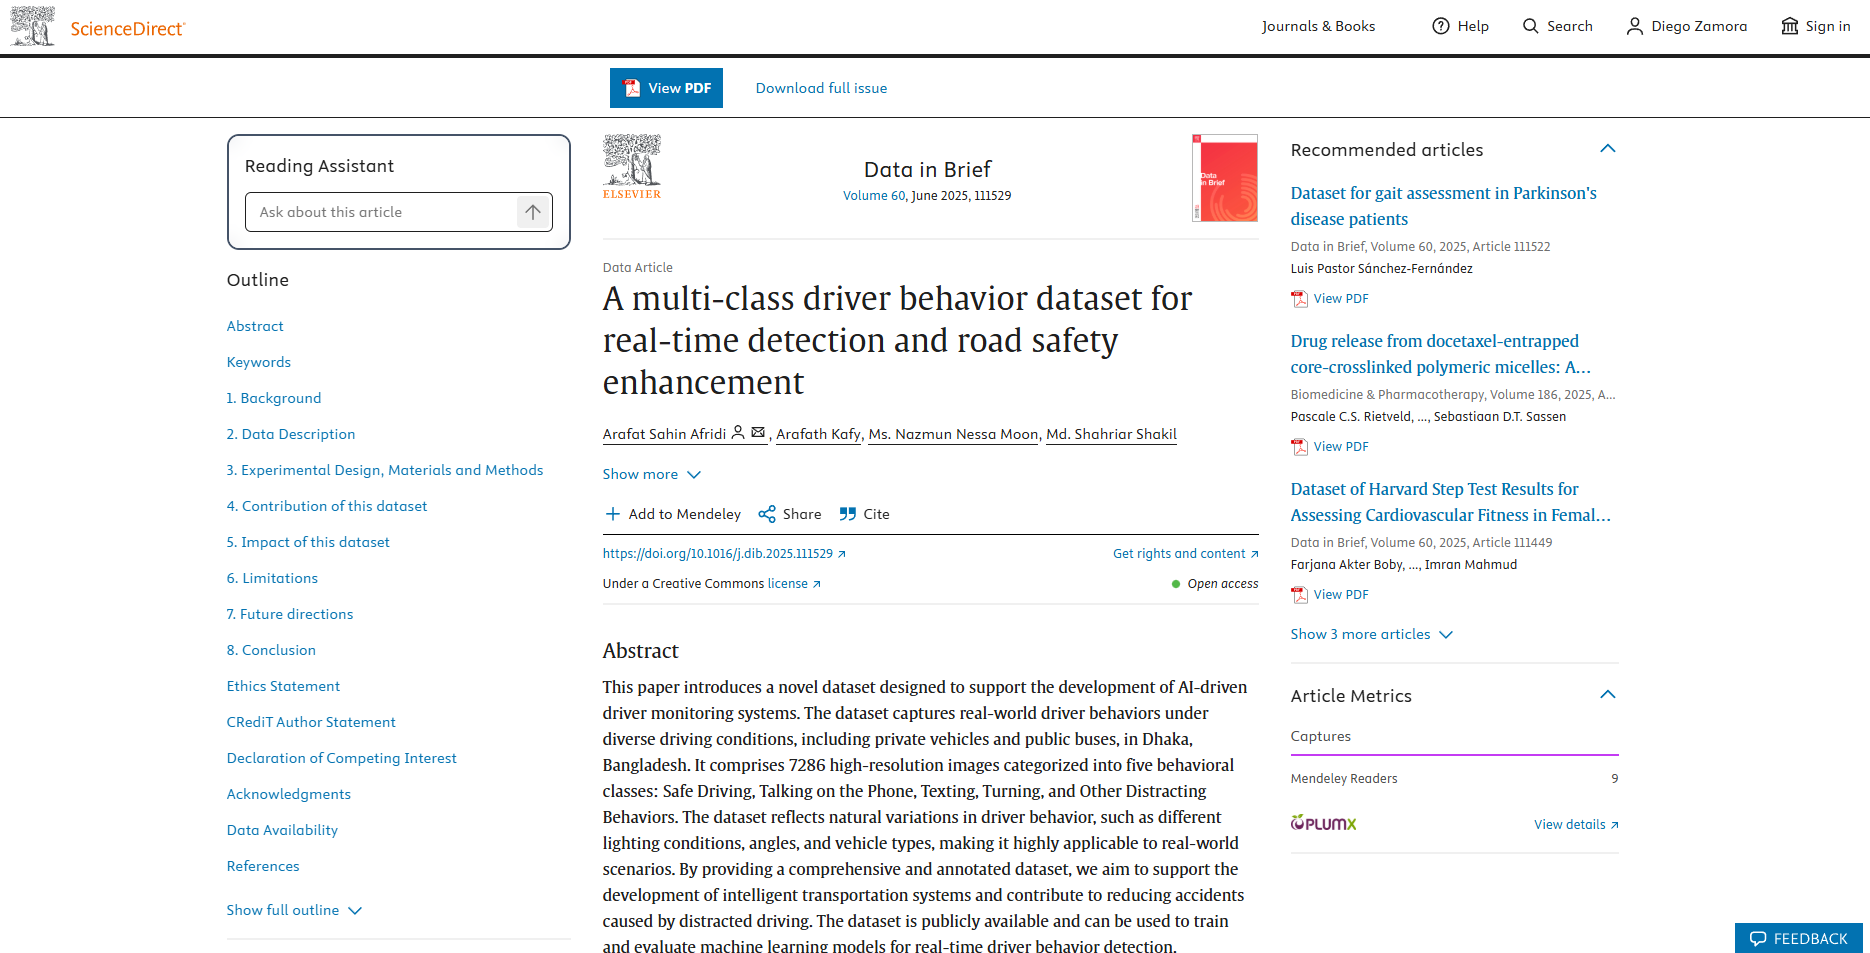
\includegraphics[width=\linewidth]{Anexo/Captura 7.png}
			\caption{A multi-class driver behavior dataset for real-time detection and road safety enhancement}
		\end{minipage}
	\end{figure}
	\subsection{Guía de Entrevista Estructurada}
	
	La siguiente guía fue utilizada durante el proceso de elicitación para obtener información relevante de conductores e instructores de conducción.
	
	\textbf{Objetivo:} Identificar necesidades funcionales y restricciones del sistema desde la perspectiva de conductores e instructores.
	
	\begin{enumerate}
		\item ¿Cuáles son los errores más frecuentes en conductores en formación?
		\item ¿Qué situaciones críticas deberían simularse prioritariamente?
		\item ¿Qué métricas considera importantes para evaluar desempeño?
		\item ¿Qué tipo de retroalimentación resulta más efectiva?
		\item ¿Qué expectativas tiene respecto al realismo del simulador?
		\item ¿Qué requisitos de seguridad considera necesarios?
		\item ¿Qué dificultades observa en la enseñanza tradicional?
		\item ¿Qué funcionalidades administrativas considera necesarias?
		\item ¿Qué tipo de reportes debería generar el sistema?
		\item ¿Qué aspectos tecnológicos podrían mejorar la experiencia?
	\end{enumerate}

    % =====================================================
\subsubsection{Repositorio del Proyecto}
% =====================================================

Con el propósito de garantizar la trazabilidad y disponibilidad del material desarrollado durante el proyecto, se dispone de un repositorio público donde se almacenan evidencias relevantes del trabajo realizado.

El repositorio puede consultarse en el siguiente enlace:

\begin{center}
\href{https://github.com/MoisesPanama/INGENIER-A-DE-REQUERIMIENTOS}{https://github.com/MoisesPanama/INGENIER-A-DE-REQUERIMIENTOS}
\end{center}

	% =====================================================
\subsection{Prototipo de Baja y Alta Fidelidad}
% =====================================================

En esta sección se presentan las interfaces correspondientes al prototipo del sistema desarrollado durante la fase de diseño. Se incluyen tanto los bocetos iniciales de baja fidelidad como las interfaces de alta fidelidad, las cuales permiten visualizar la evolución del diseño de la aplicación.

% =====================================================
\subsubsection{Prototipo de Baja Fidelidad}
% =====================================================

El prototipo de baja fidelidad corresponde a una serie de bocetos iniciales que representan de manera conceptual la estructura de las interfaces del sistema. Estos diseños permiten validar la organización de los elementos, la navegación y la interacción básica del usuario antes de desarrollar versiones más detalladas del sistema.

\begin{figure}[H]
\centering
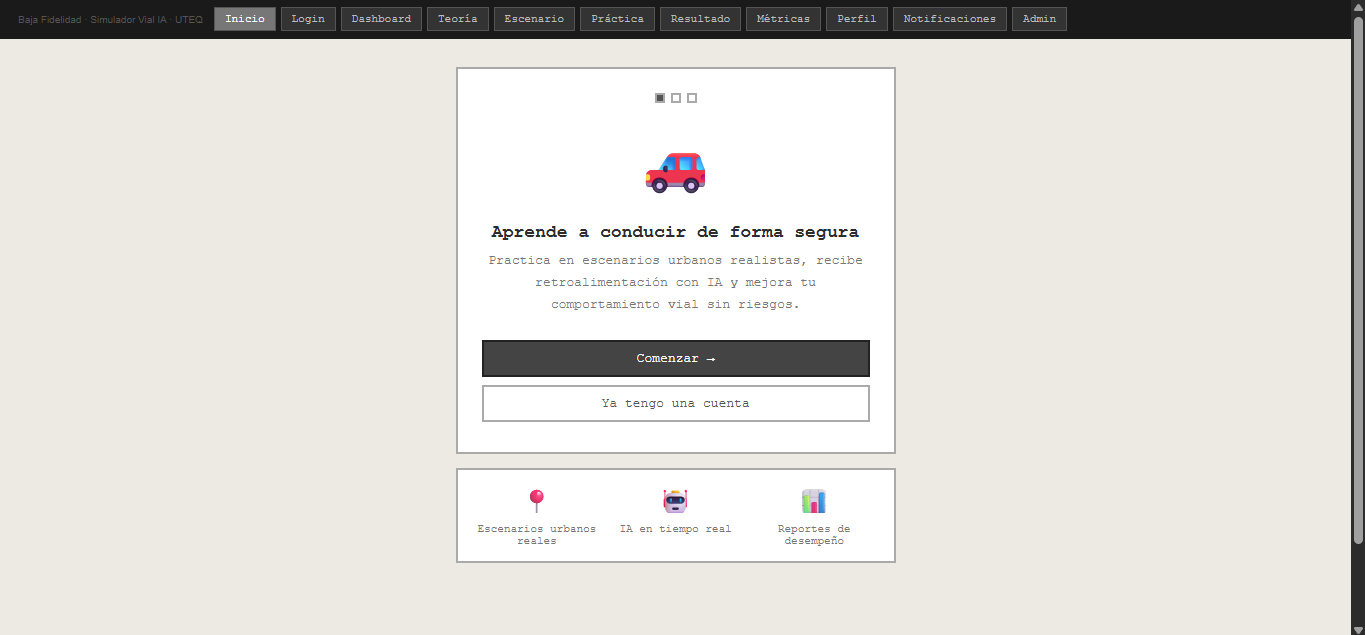
\includegraphics[width=0.8\textwidth]{Prototipo/bf1.png}
\caption{Prototipo de baja fidelidad – Pantalla 1}
\end{figure}

\begin{figure}[H]
\centering
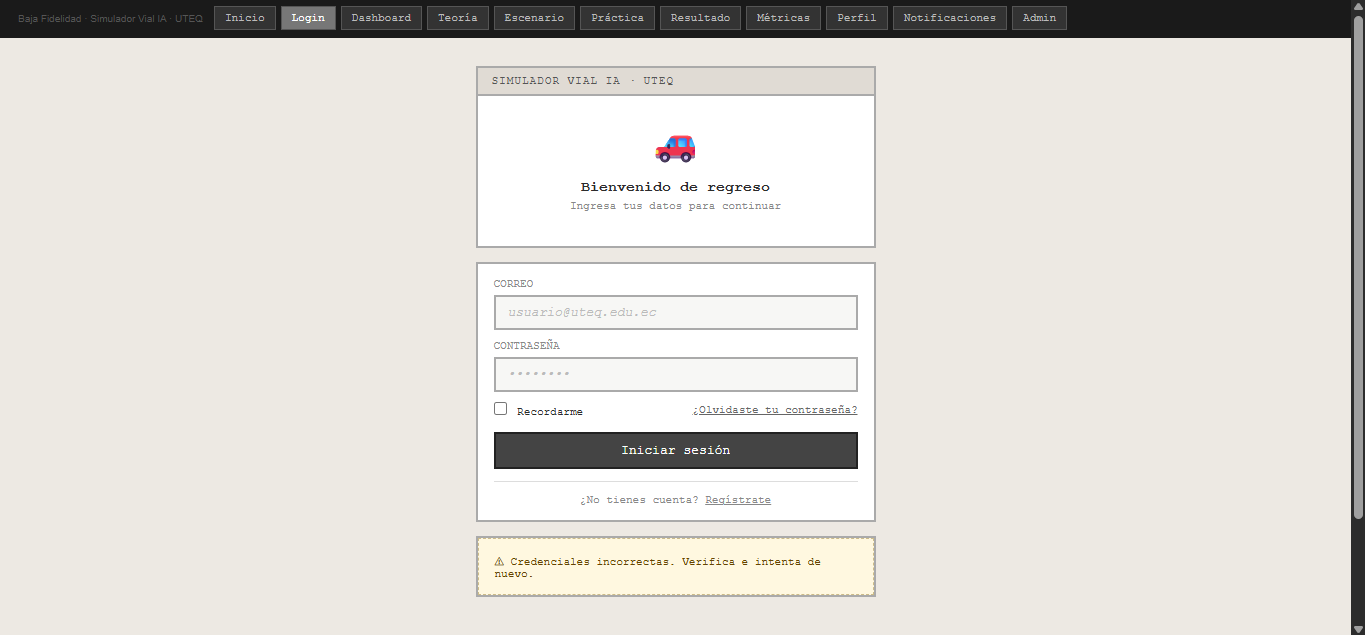
\includegraphics[width=0.8\textwidth]{Prototipo/bf2.png}
\caption{Prototipo de baja fidelidad – Pantalla 2}
\end{figure}

\begin{figure}[H]
\centering
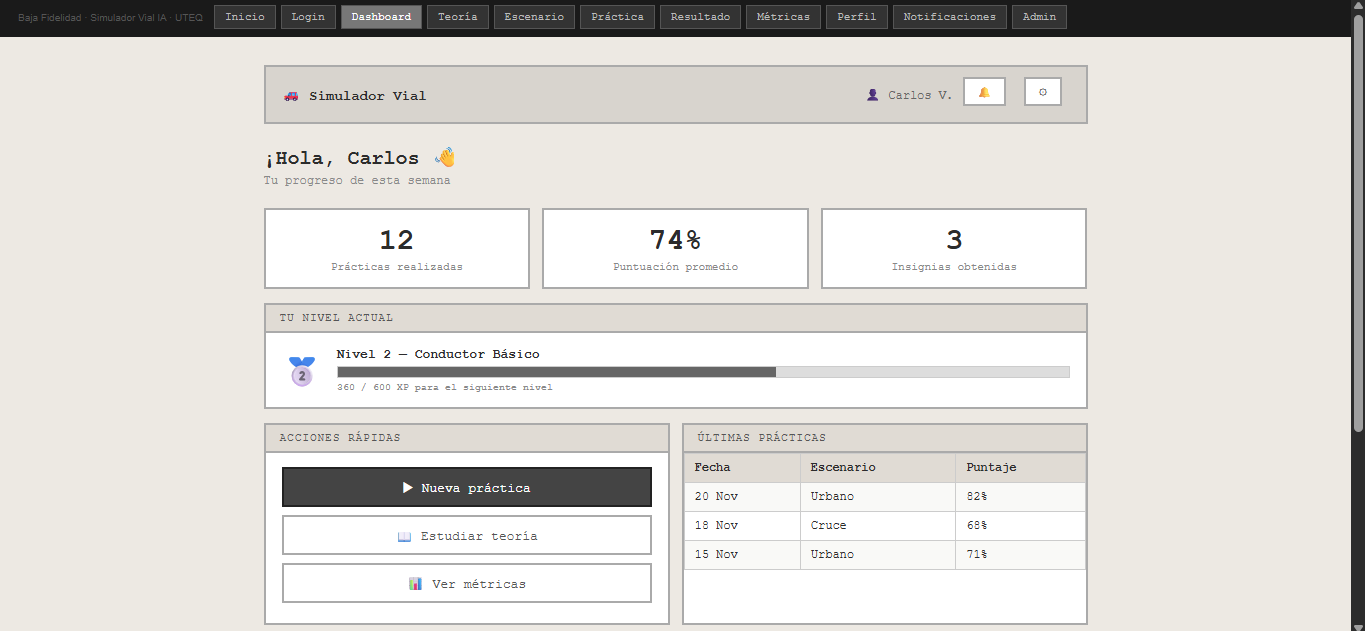
\includegraphics[width=0.8\textwidth]{Prototipo/bf3.png}
\caption{Prototipo de baja fidelidad – Pantalla 3}
\end{figure}

\begin{figure}[H]
\centering
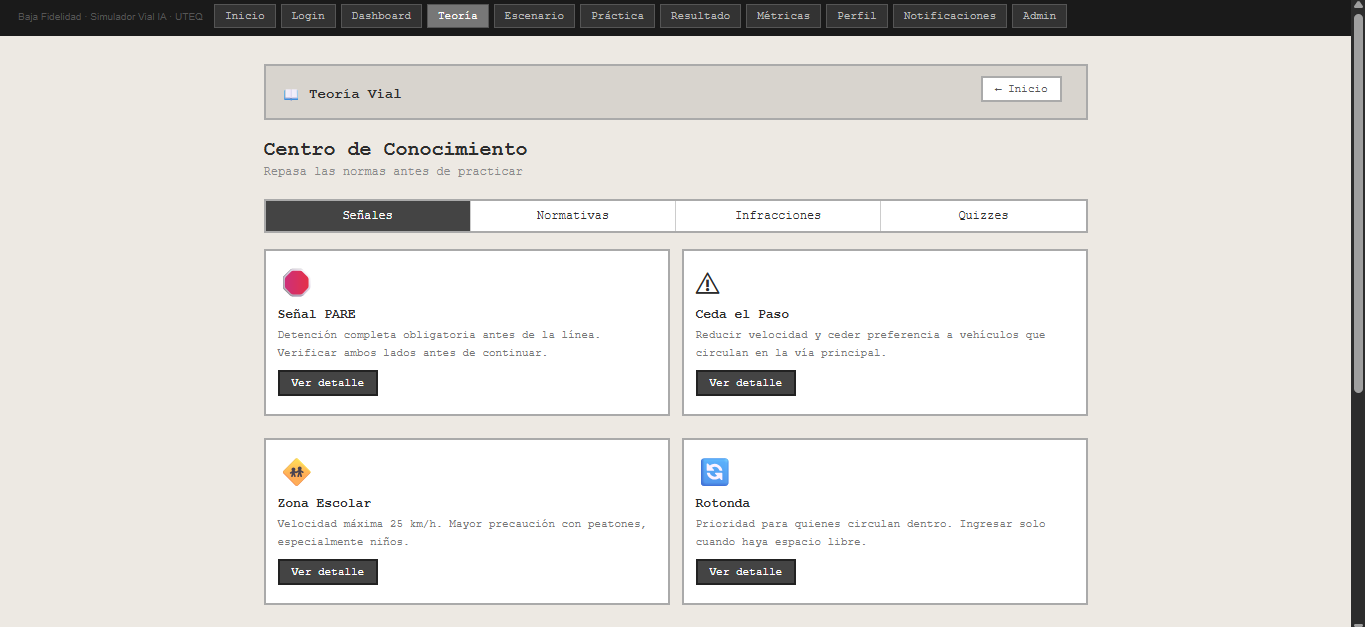
\includegraphics[width=0.8\textwidth]{Prototipo/bf4.png}
\caption{Prototipo de baja fidelidad – Pantalla 4}
\end{figure}

\begin{figure}[H]
\centering
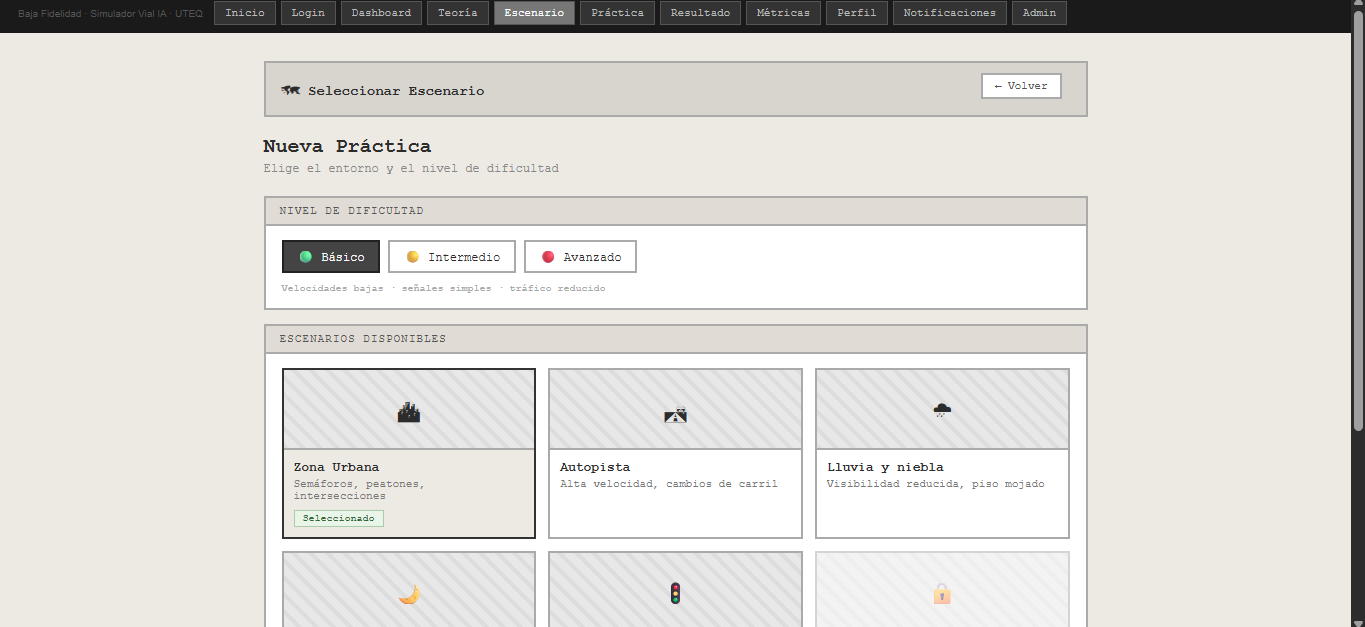
\includegraphics[width=0.8\textwidth]{Prototipo/bf5.png}
\caption{Prototipo de baja fidelidad – Pantalla 5}
\end{figure}

\begin{figure}[H]
\centering
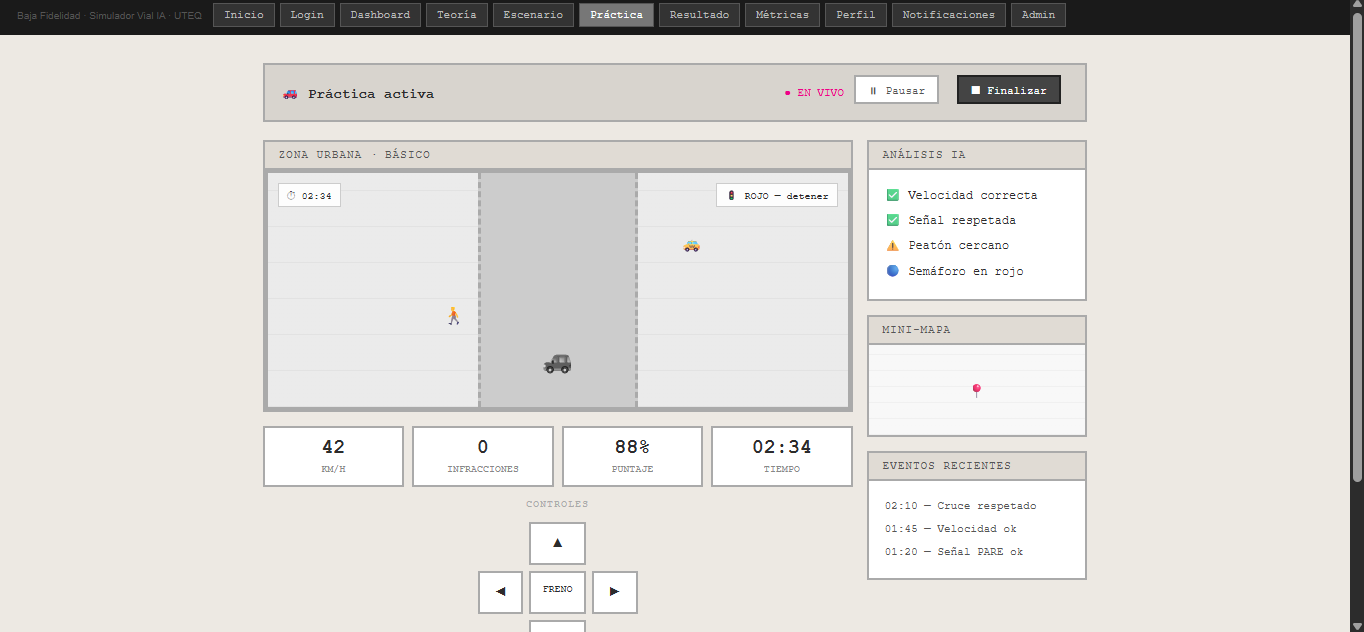
\includegraphics[width=0.8\textwidth]{Prototipo/bf6.png}
\caption{Prototipo de baja fidelidad – Pantalla 6}
\end{figure}

\begin{figure}[H]
\centering
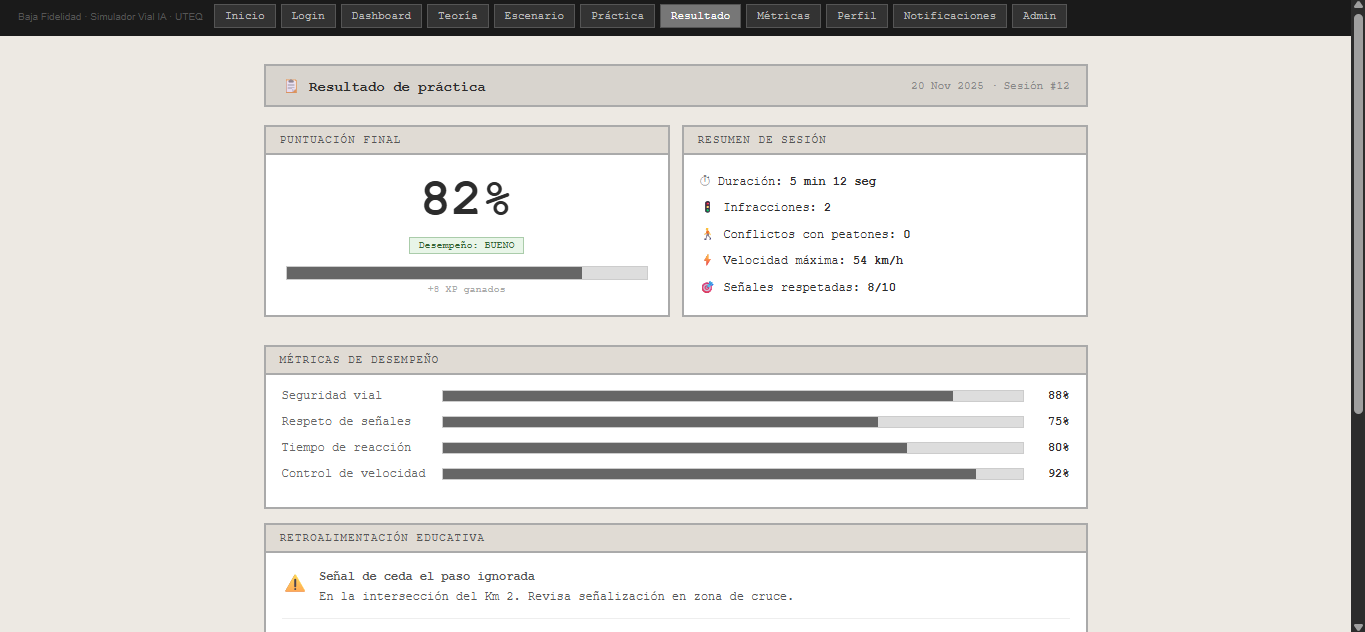
\includegraphics[width=0.8\textwidth]{Prototipo/bf7.png}
\caption{Prototipo de baja fidelidad – Pantalla 7}
\end{figure}

\begin{figure}[H]
\centering
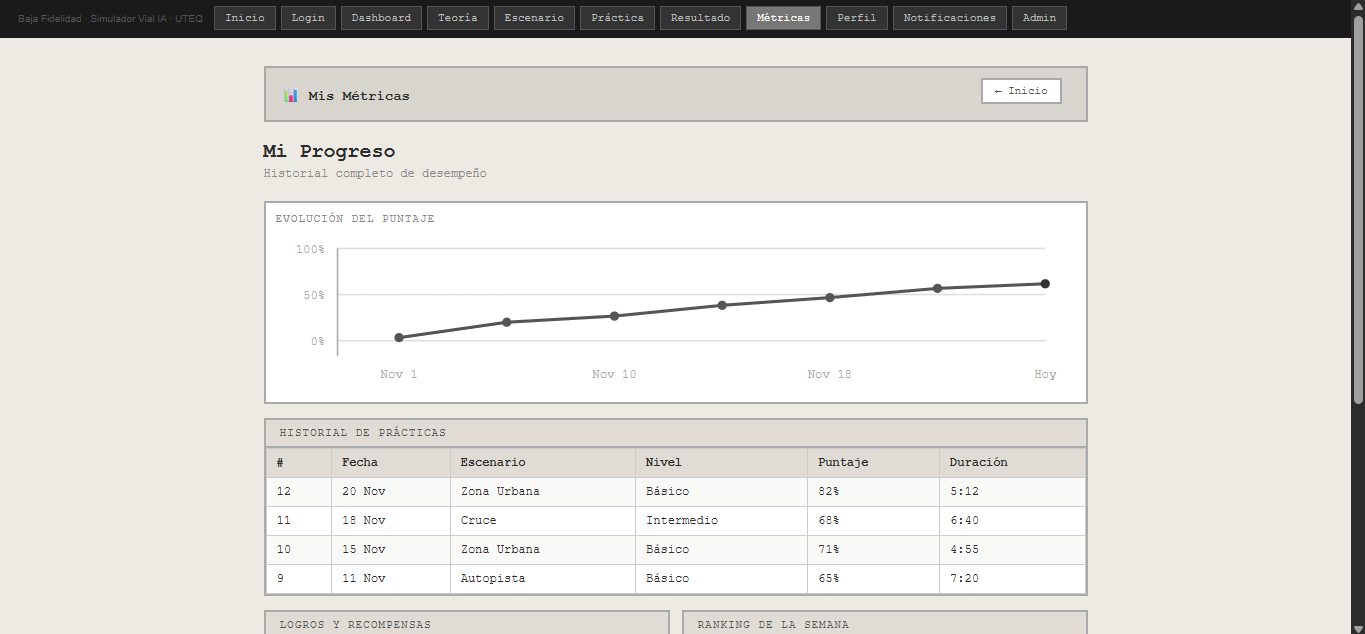
\includegraphics[width=0.8\textwidth]{Prototipo/bf8.png}
\caption{Prototipo de baja fidelidad – Pantalla 8}
\end{figure}

\begin{figure}[H]
\centering
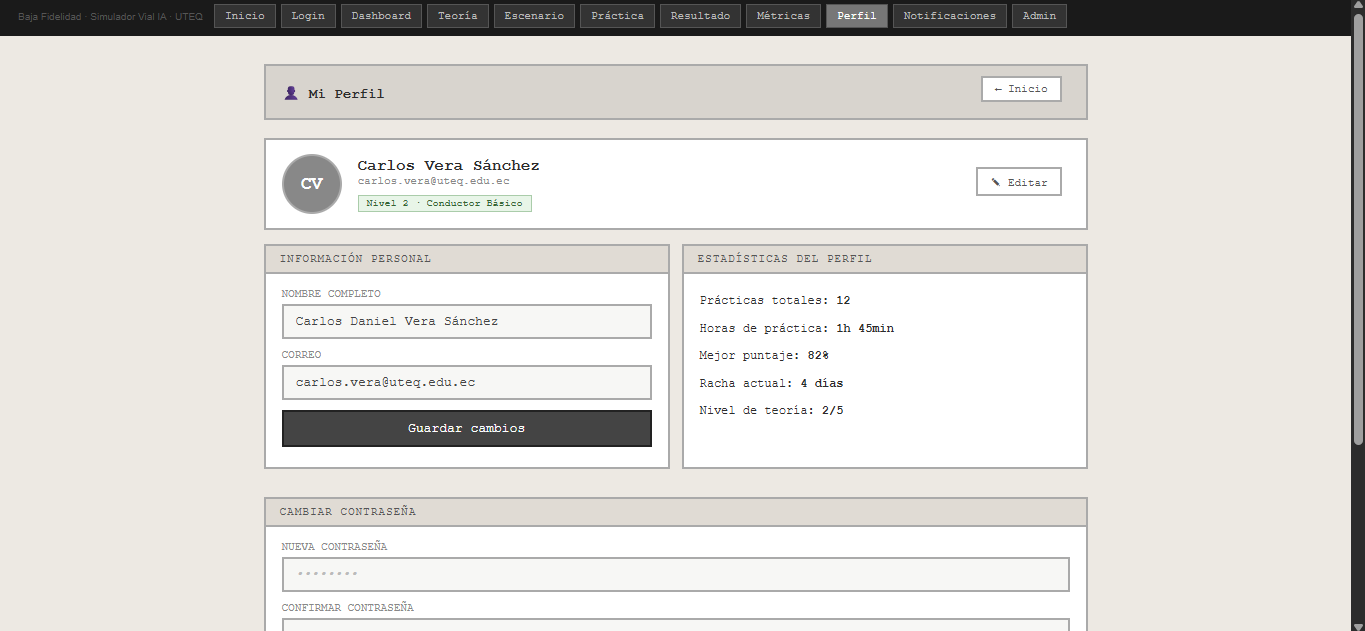
\includegraphics[width=0.8\textwidth]{Prototipo/bf9.png}
\caption{Prototipo de baja fidelidad – Pantalla 9}
\end{figure}

\begin{figure}[H]
\centering
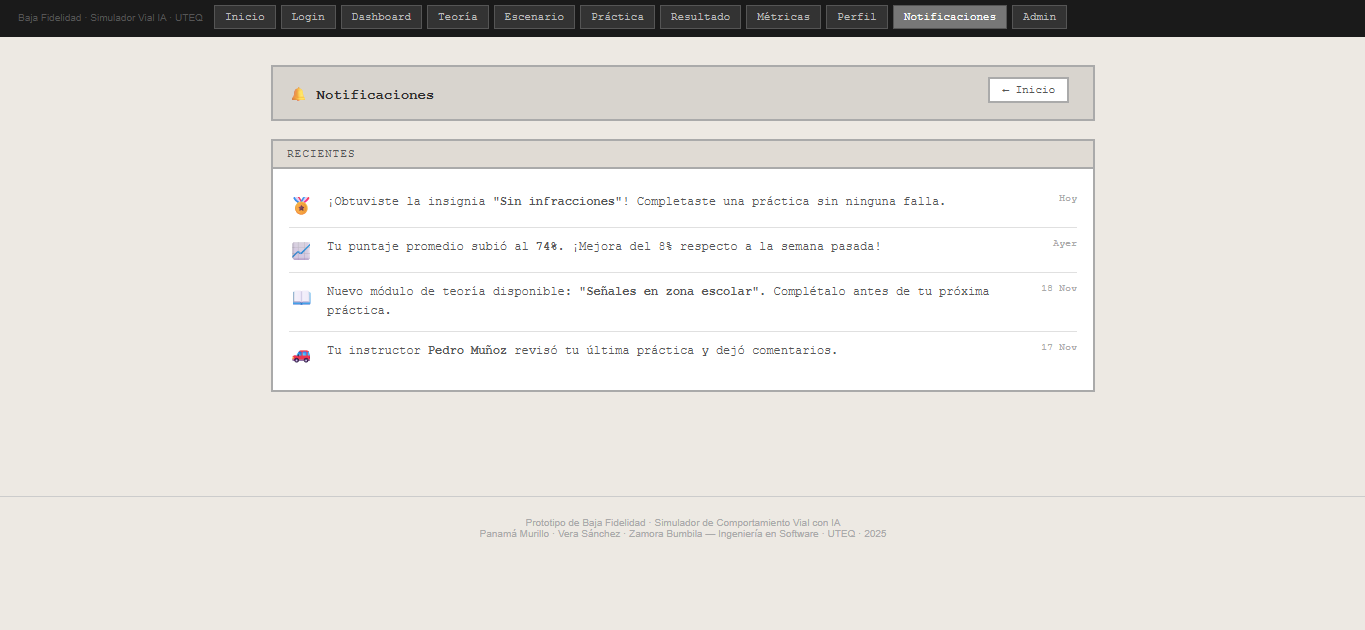
\includegraphics[width=0.8\textwidth]{Prototipo/bf10.png}
\caption{Prototipo de baja fidelidad – Pantalla 10}
\end{figure}

\begin{figure}[H]
\centering
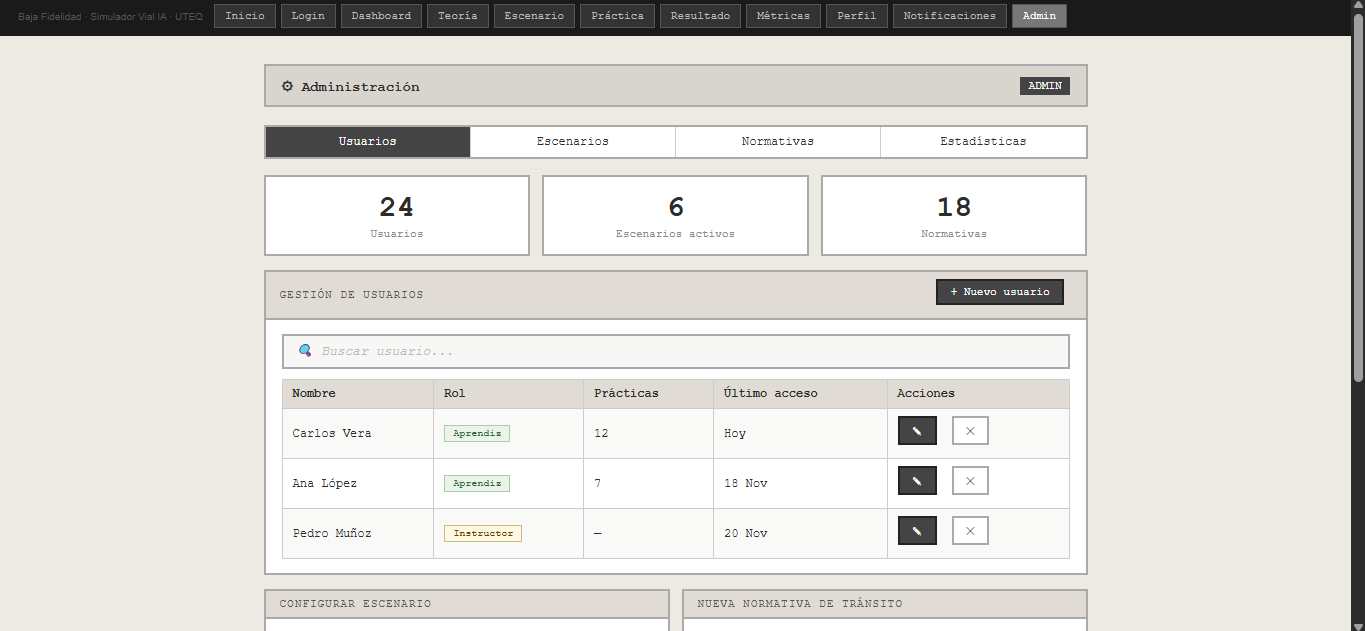
\includegraphics[width=0.8\textwidth]{Prototipo/bf11.png}
\caption{Prototipo de baja fidelidad – Pantalla 11}
\end{figure}


% =====================================================
\subsubsection{Prototipo de Alta Fidelidad}
% =====================================================

El prototipo de alta fidelidad representa una versión más detallada de las interfaces del sistema, incorporando elementos visuales, estructura de navegación y componentes gráficos más cercanos al diseño final de la aplicación. Estas interfaces permiten evaluar de forma más precisa la experiencia de usuario y la interacción con las funcionalidades principales del simulador.

\begin{figure}[H]
\centering
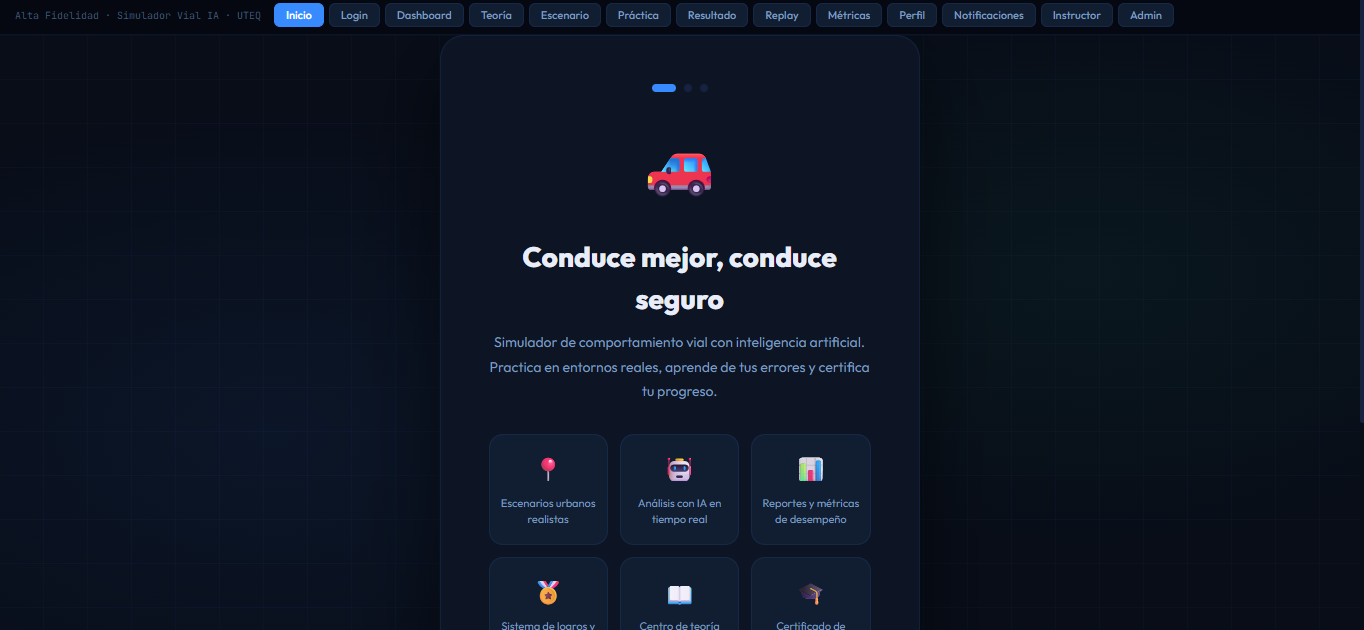
\includegraphics[width=0.8\textwidth]{Prototipo/af1.png}
\caption{Prototipo de alta fidelidad – Pantalla 1}
\end{figure}

\begin{figure}[H]
\centering
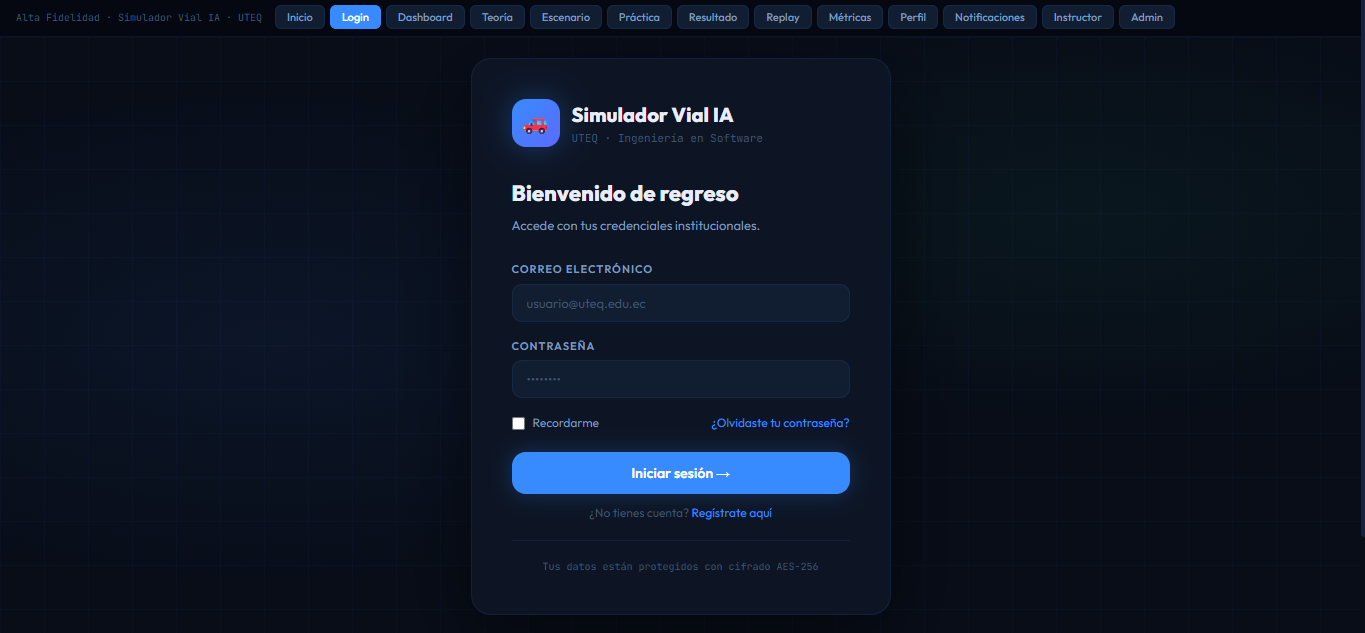
\includegraphics[width=0.8\textwidth]{Prototipo/af2.png}
\caption{Prototipo de alta fidelidad – Pantalla 2}
\end{figure}

\begin{figure}[H]
\centering
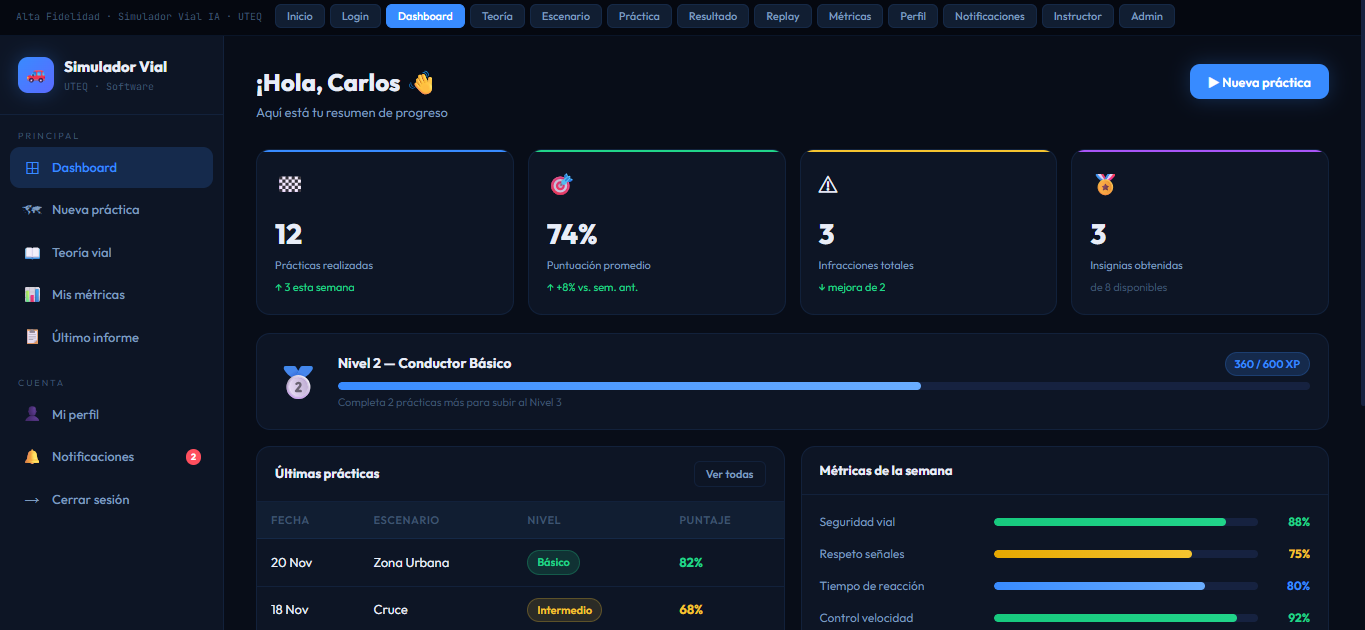
\includegraphics[width=0.8\textwidth]{Prototipo/af3.png}
\caption{Prototipo de alta fidelidad – Pantalla 3}
\end{figure}

\begin{figure}[H]
\centering
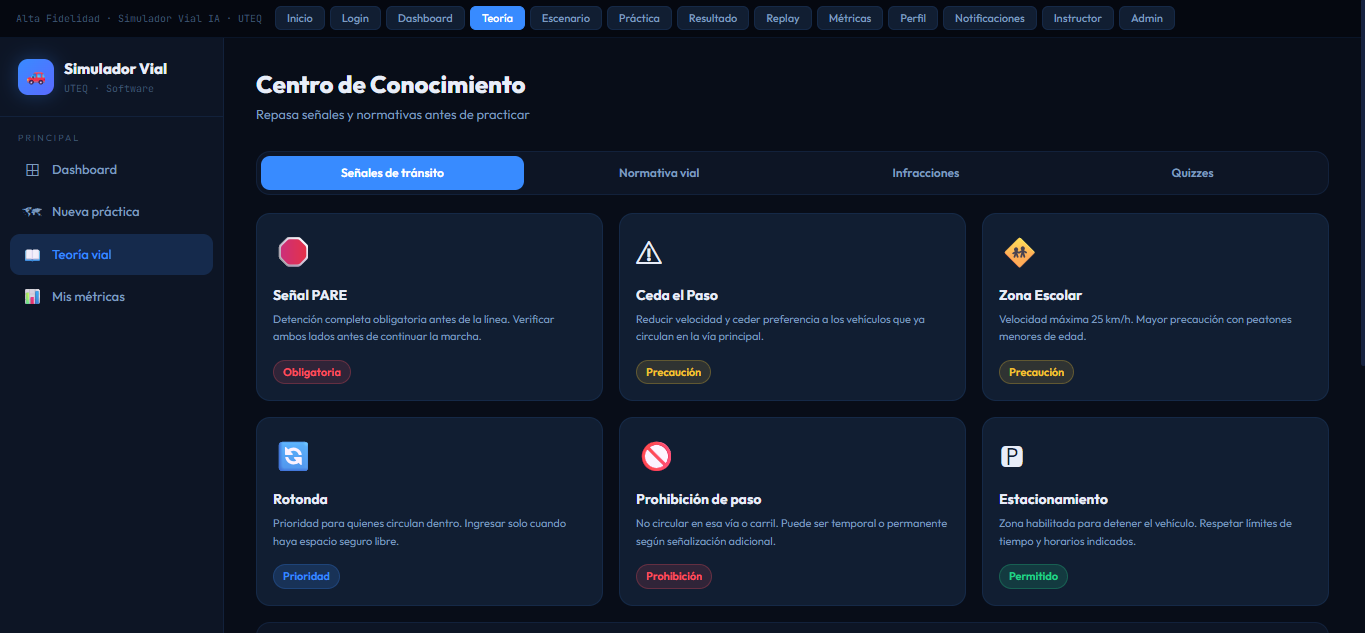
\includegraphics[width=0.8\textwidth]{Prototipo/af4.png}
\caption{Prototipo de alta fidelidad – Pantalla 4}
\end{figure}

\begin{figure}[H]
\centering
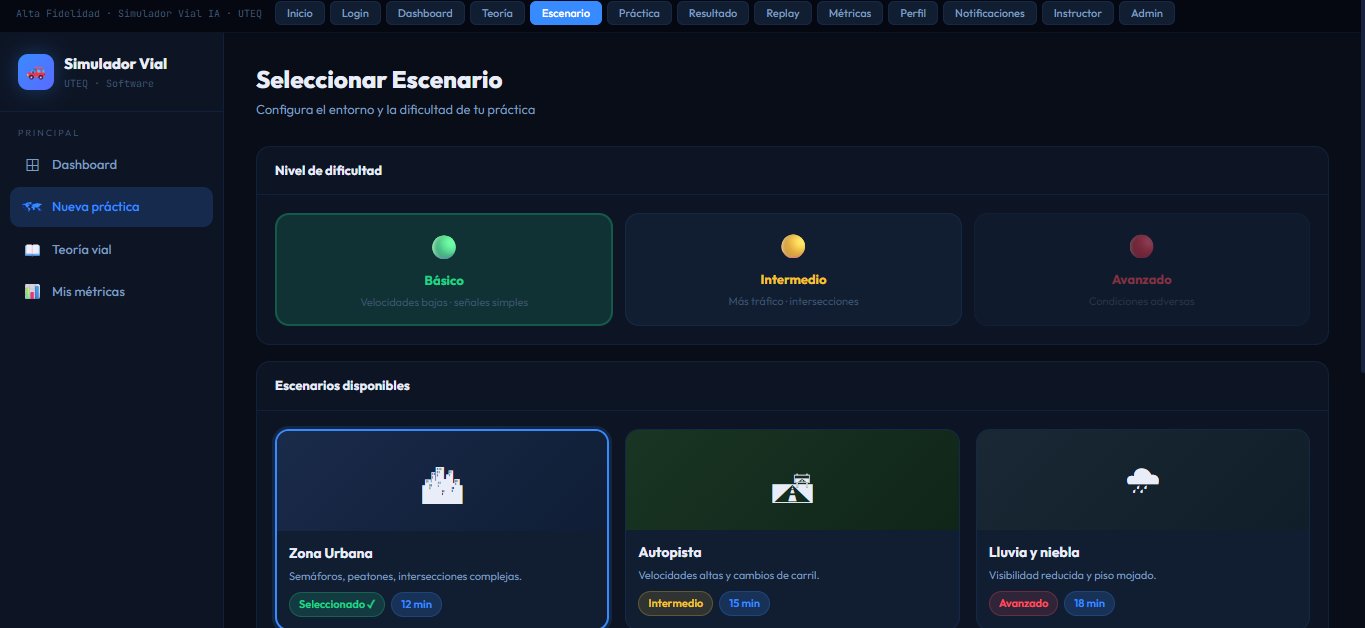
\includegraphics[width=0.8\textwidth]{Prototipo/af5.png}
\caption{Prototipo de alta fidelidad – Pantalla 5}
\end{figure}

\begin{figure}[H]
\centering
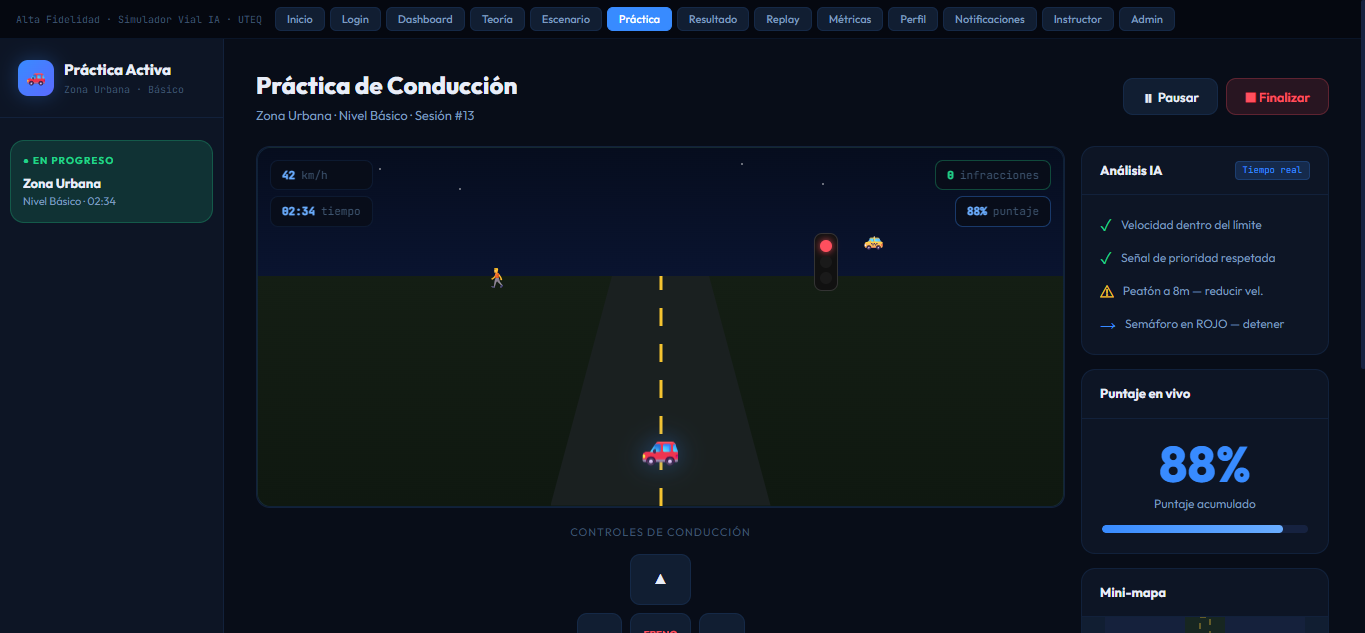
\includegraphics[width=0.8\textwidth]{Prototipo/af6.png}
\caption{Prototipo de alta fidelidad – Pantalla 6}
\end{figure}

\begin{figure}[H]
\centering
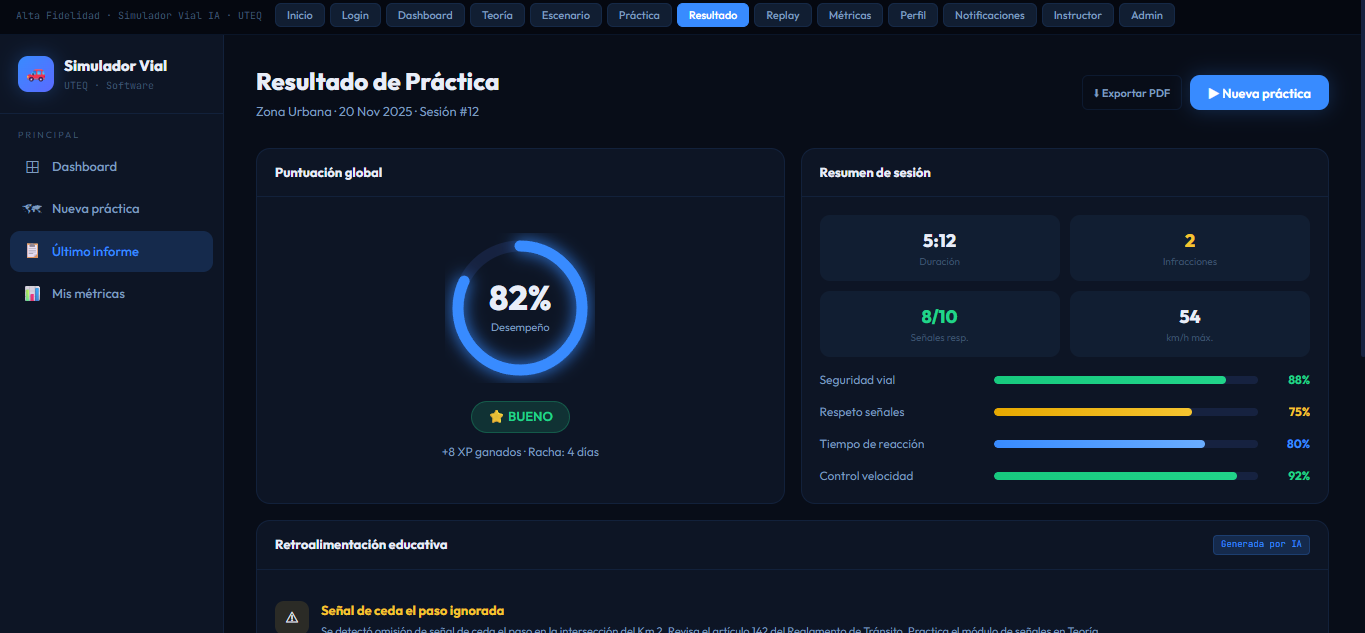
\includegraphics[width=0.8\textwidth]{Prototipo/af7.png}
\caption{Prototipo de alta fidelidad – Pantalla 7}
\end{figure}

\begin{figure}[H]
\centering
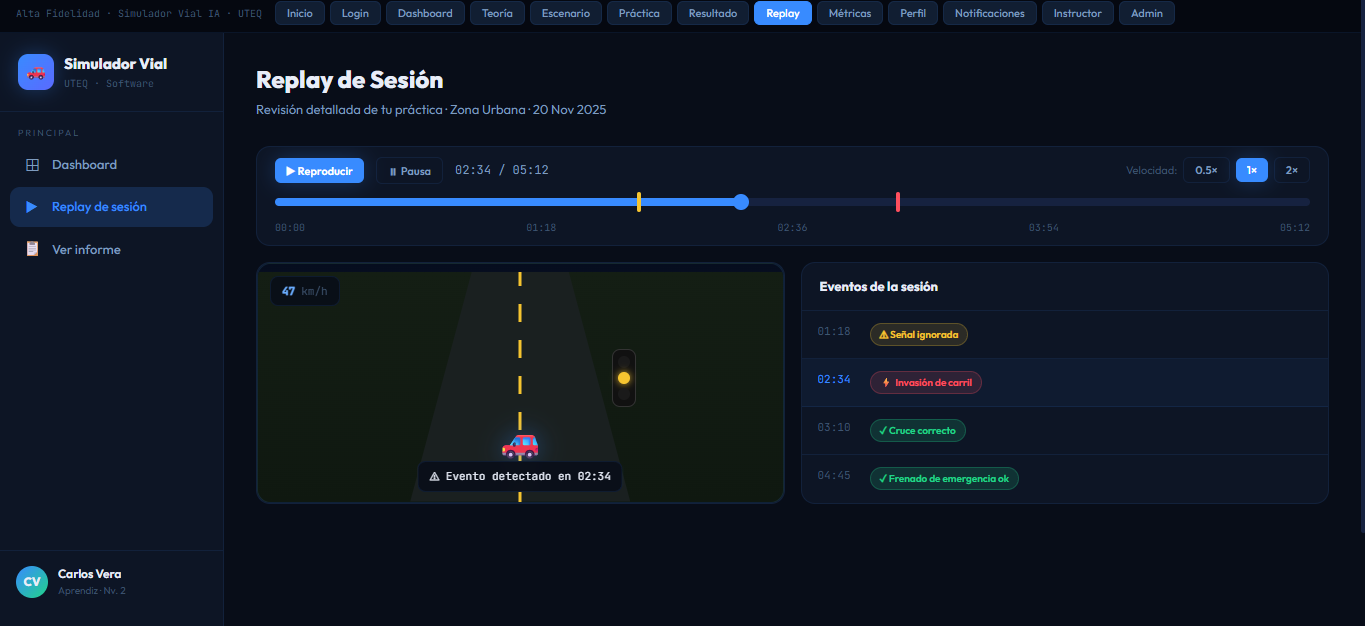
\includegraphics[width=0.8\textwidth]{Prototipo/af8.png}
\caption{Prototipo de alta fidelidad – Pantalla 8}
\end{figure}

\begin{figure}[H]
\centering
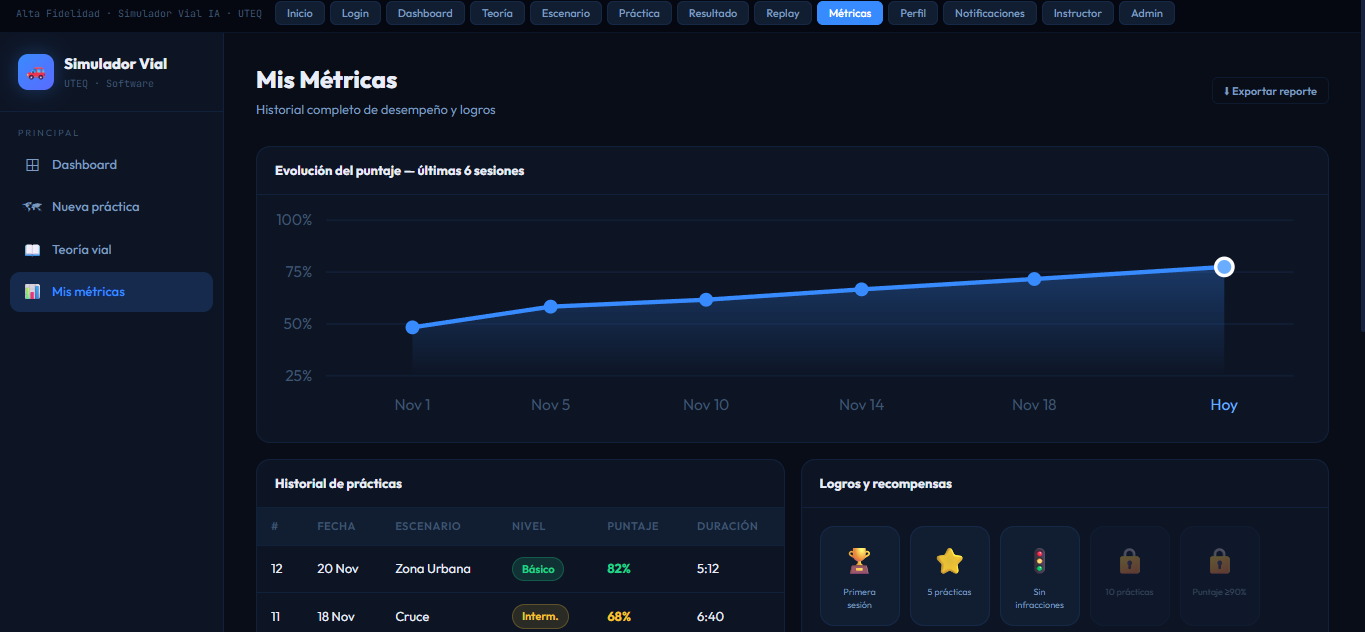
\includegraphics[width=0.8\textwidth]{Prototipo/af9.png}
\caption{Prototipo de alta fidelidad – Pantalla 9}
\end{figure}

\begin{figure}[H]
\centering
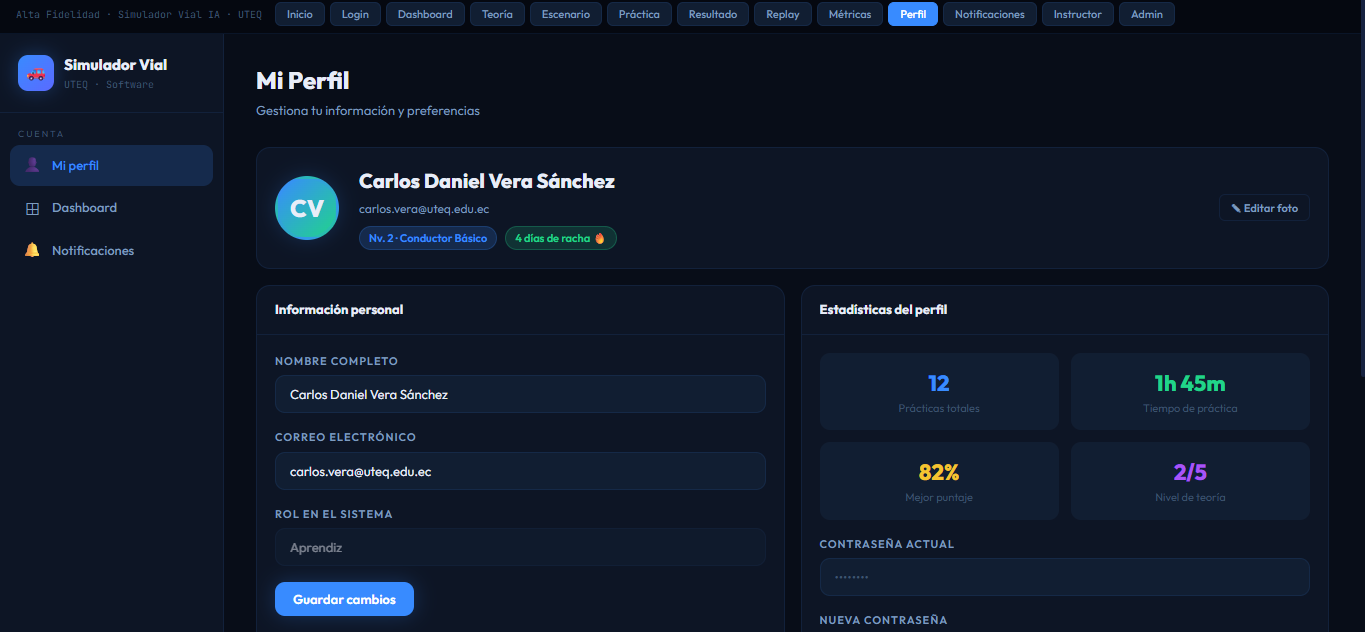
\includegraphics[width=0.8\textwidth]{Prototipo/af10.png}
\caption{Prototipo de alta fidelidad – Pantalla 10}
\end{figure}

\begin{figure}[H]
\centering
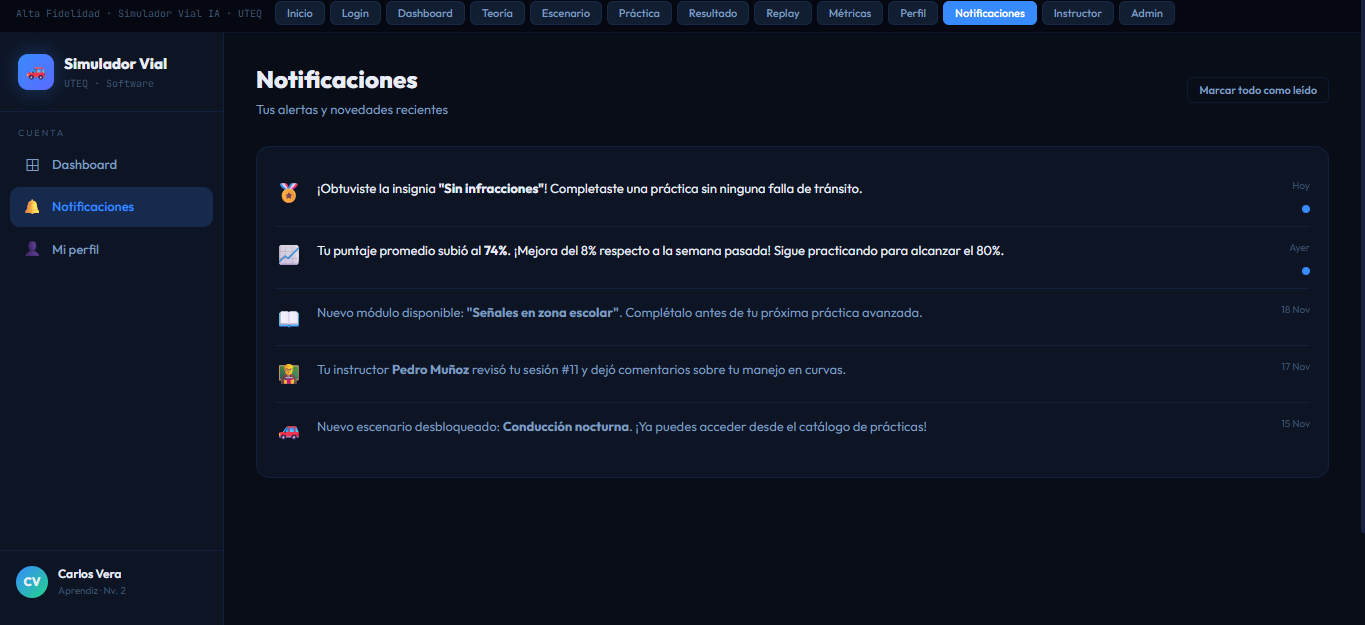
\includegraphics[width=0.8\textwidth]{Prototipo/af11.png}
\caption{Prototipo de alta fidelidad – Pantalla 11}
\end{figure}

\begin{figure}[H]
\centering
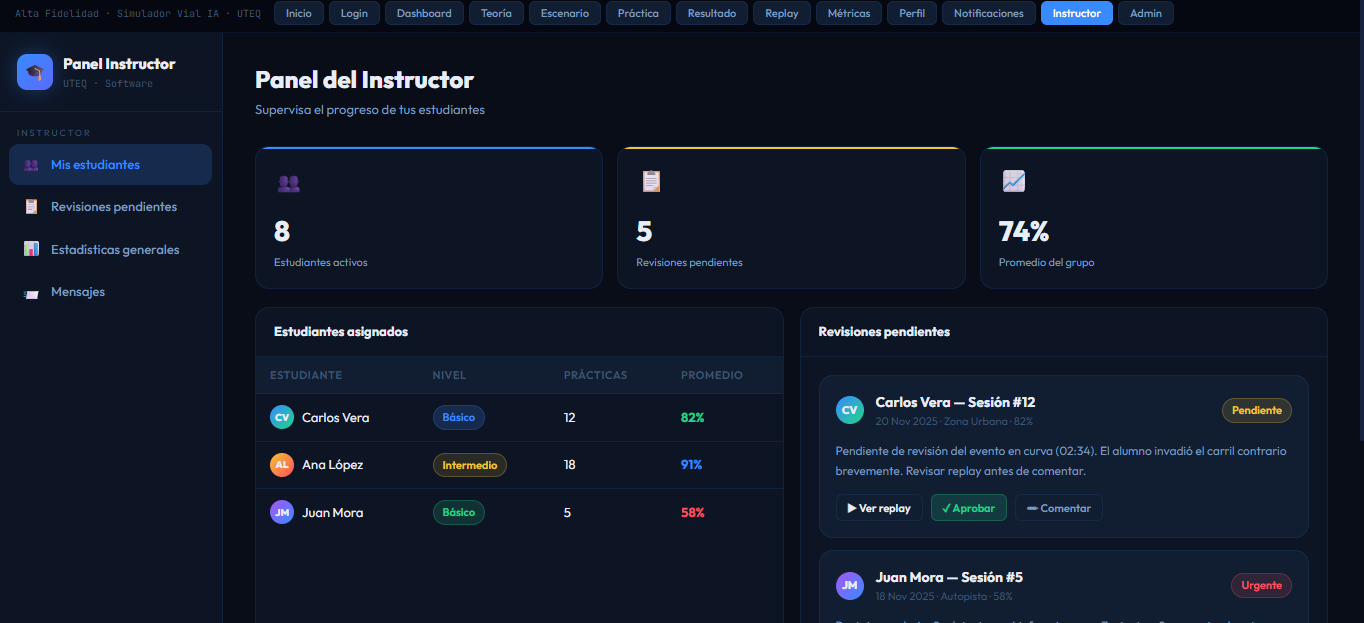
\includegraphics[width=0.8\textwidth]{Prototipo/af12.png}
\caption{Prototipo de alta fidelidad – Pantalla 12}
\end{figure}

\begin{figure}[H]
\centering
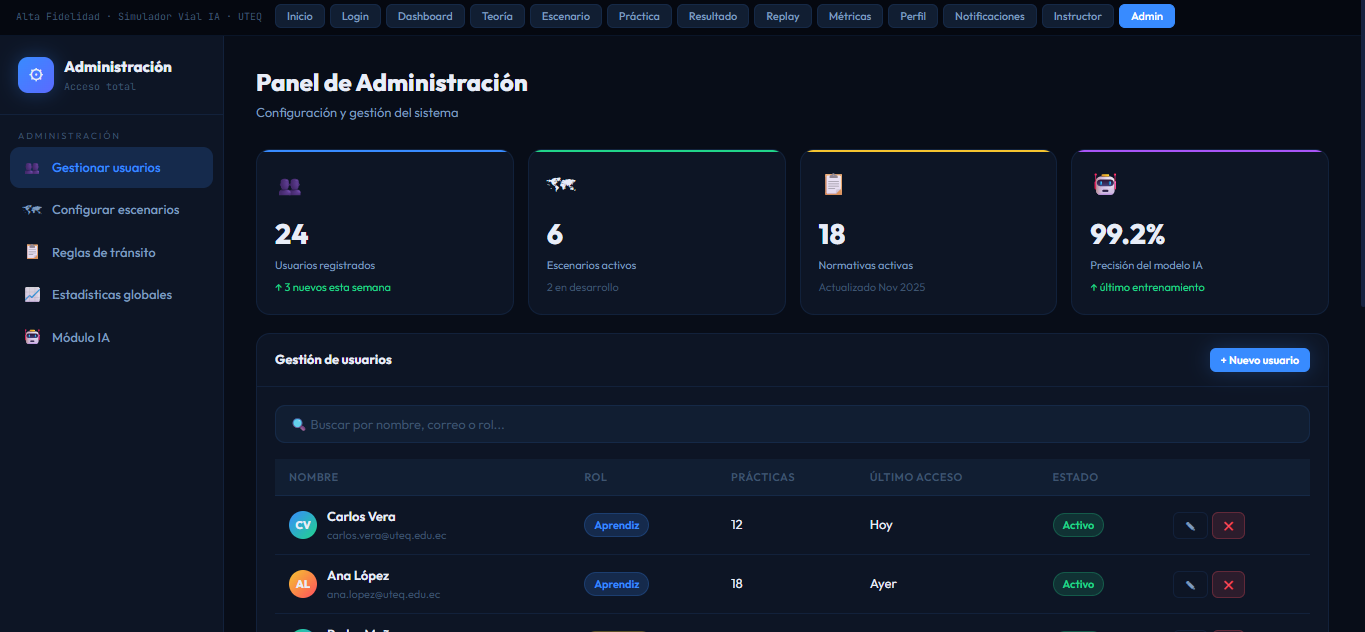
\includegraphics[width=0.8\textwidth]{Prototipo/af13.png}
\caption{Prototipo de alta fidelidad – Pantalla 13}
\end{figure}
\end{document}